\chapter{Desarrollo del TFG}
\label{ch:desarrollo}

\section{Metodología empleada: Scrum} 
\label{sec:metodologia-empleada}

Durante el desarrollo de este trabajo de fin de grado se ha hecho uso de una metodología Scrum \cite{andrewlittlefield2018}. Sin embargo, este sistema no se ha aplicado de forma estricta, si no que se han modificado algunos aspectos, adaptándolo a las necesidades que este trabajo de fin de grado ha requerido, tal como puede observarse en las siguientes líneas. 

\textbf{\large Backlog}
Este modelo comienza con un Product Owner, que es la persona que define cual será el resultado final esperado. En este caso, esta figura es personificada por el tutor de este TFG, Francisco Moya. Esta persona es también la encargada de definir el Backlog, que es la lista de tareas que serán necesarias para la realización completa del proyecto. En este caso, el Backlog ha sido elaborado por el tutor y el alumno.
Resulta de vital importancia que en el Backlog destaquen las prioridades, de manera que se resalte la importancia de aquellas tareas que implican una mayor responsabilidad a la hora de tener el producto final esperado.

\textbf{\large Sprint}
De forma posterior al Backlog, vendría el Sprint. En esta etapa se materializan los objetivos definidos previamente en el apartado Backlog. Cada etapa de Sprint debe finalizar con una revisión en la que los miembros del equipo discutan las formas de mejorar el proceso de ejecución. En nuestro TFG, la etapa de Sprint se ha dividido en dos partes principales:
\begin{enumerate}
\item \underline{ToDo.} Esta parte recoge todas las tareas extraídas del Backlog, que están por hacer. Es un punto decisivo para determinar la prioridad de cada una de las actividades, ya que aquellas que resulten de mayor interés serán transportadas al siguiente punto, donde se ejecutarán.
\item \underline{Doing.} Las tareas que se encuentran en este punto se encuentran en proceso de materialización. El apartado Doing implica el ecuador de este modelo de trabajo, ya que es el instante en el que se llevan a efecto los trabajos, que en conjunto, determinarán el resultado final del proyecto.
\end{enumerate}

\textbf{\large Quality Control}
Una vez que las tareas han sido realizadas en el apartado de Sprint, se procede a transportarlas hacia el Quality Control, o control de calidad, donde se hará un análisis sistemático de las mismas, en el que se determinará si estas han cumplido o no con los criterios exigidos. Durante el transcurso de este trabajo de fin de grado, el tutor Francisco Moya, ha sido quien ha trabajado este apartado aceptando, rechazando o proponiendo modificaciones siempre que lo ha considerado necesario. Del resultado de estas valoraciones se determinará si la tarea ha sido completada correctamente, o si por el contrario, necesita ser editada o replanteada.

\textbf{\large Done}
Una tarea acaba en el apartado Done cuando esta ha sido aceptada en su proceso de control de calidad. Que una tarea ocupe esta posición significa que no necesita más ediciones ni tampoco más revisiones, por lo que puede considerarse que se encuentra completamente terminada.

\textbf{\large Blocked}
El apartado Blocked comprende uno de los aspectos más importantes de la metodología Scrum. Cuando una tarea no puede ser completada, por cualquier circunstancia, se puede transportar a este apartado, donde un miembro o un equipo de jerarquía superior podrá determinar una solución. En el caso de este trabajo de fin de grado, el tutor Francisco Moya ha sido quien ha ido determinando las soluciones que se debían proponer a los problemas que el alumno ha ido transportando a esta posición.
\section{Planificación del proyecto} 
\label{sec:planificacion-del-proyecto}
Una vez definidos debidamente los objetivos y la metodología de trabajo, se procede a determinar cuál será la planificación del proyecto. Esta planificación implica la división que se ha realizado sobre el problema que se aborda, en todas las fases necesarias para la obtención de una solución satisfactoria y definitiva.

Este problema se afronta desde la división de 3 fases principales: circuito electrónico, diseño de algoritmos y programación, y por último, seguridad. Cada una de estas fases guarda dependencias entre sí, por lo que su ejecución no puede ser completamente independiente ni ir en un marco temporal diferente. La seguridad, por ejemplo, contempla uno de los aspectos más importantes a tener en cuenta en el proyecto, y aunque los trabajos de programación referidos a este apartado y las revisiones y modificaciones han venido al final del proyecto, todos los trabajos realizados anteriormente, en cualquiera de las fases, han tenido en cuenta este y otros factores. A continuación se definen, a través de las 3 fases principales, las tareas que se han propuesto durante el desarrollo de este trabajo de fin de grado.
\subsection{Construcción del circuito electrónico} 
El modelo de portero automático con el que se ha trabajado en este proyecto, es el FERMAX 8044, cuyas características técnicas se especificarán más adelante. Teniendo esto en cuenta, los trabajos orientados al desarrollo del circuito electrónico han debido adaptarse al funcionamiento de este modelo.

La primera parte del trabajo ha consistido, por tanto, en tratar de activar la apertura de una cerradura eléctrica, por medio de un portero automático, activado con una señal emitida por una Raspberry Pi Zero W. Para la consecución de esta tarea se han programado tareas de distinto ámbito, como son las siguientes:
\begin{enumerate}
\item \underline{Documentación de los elementos a emplear:} En primer lugar, con el fin de adquirir la información necesaria para llevar a cabo la ejecución correcta del circuito electrónico, se ha elaborado una tarea consistente en estudiar el funcionamiento de cada uno de los componentes que serán precisos.
\item \underline{Conexiones físicas:} Estas tarea consiste en determinar que elementos serán necesarios para el correcto funcionamiento del circuito, y una vez que este haya sido construido, en realizar la conexión de estos elementos.
\item \underline{Fijación de los elementos} Para que el transporte físico del prototipo sea seguro, se ha decidido incluir una tarea en este apartado con la que se garantice una sujeción firme.
\end{enumerate}
\subsection{Diseño de algoritmos y programación}
Sin duda, el grueso de este trabajo de fin de grado corresponde a la realización de todos los programas que permitirán el correcto cumplimiento de los objetivos definidos.
Esta tarea se ha dividido a su vez en diferentes subtareas, las cuales se definen a continuación:
\begin{enumerate}

\item \underline{Programa capaz de activar la señal:} A partir de la aplicación de mensajería instantánea "Telegram", esta tarea refiere la misión de conseguir que, a partir de una petición hecha por un usuario desde esta aplicación, se active una señal que, con el circuito elaborado previamente, active la señal que permita realizar la apertura de la puerta.
Este programa deberá incluir también un panel de administrador, con el fin de que el anfitrión tenga la posibilidad de crear accesos a la vivienda a aquellos usuarios que considere conveniente, así como cancelar estos accesos. Desde este panel, también se deberán incluir opciones de modificación de reservas y realizar las peticiones de acceso a la vivienda.
\item \underline{Programa capaz de recibir las reservas:} Esta tarea se considerará completada en el momento en que, al producirse una reserva en la plataforma de alquiler (en este proyecto se ha elegido Booking.com por ser la plataforma más utilizada en el mundo), el programa incluya la información de entrada en el sistema, y permita acceder al huésped, en la fecha definida y con su número de reserva, a la propiedad que ha alquilado.
\item \underline{Programa capaz de cancelar las reservas:} Al igual que se producen nuevas reservas, se producen cancelaciones, por lo que un sistema necesitará tenerlas en cuenta para funcionar de forma correcta. Es por ello que, en esta tarea se establece el desarrollo de un algoritmo que integre la información necesaria en el sistema al producirse una cancelación.
\item \underline{Unificar los programas anteriores:}Una vez que se cuente con los programas mencionados en los puntos anteriores, es de vital importancia hacer que funcionen de forma síncrona, por lo que el objetivo de esta tarea es el de cumplir con dicha exigencia.
\end{enumerate}
\subsection{Tareas orientadas a la seguridad del dispositivo}
Si se busca la definición de "seguro" en la Real Academia Española, podrá observarse que se define como "libre y exento de todo riesgo", y si se baja unas cuantas líneas más, encontraremos la siguiente definición: "que no falla o que ofrece confianza".
Garantizar, a día de hoy, un sistema conectado a la red que sea completamente seguro es algo prácticamente imposible para cualquier empresa. Algunas de ellas \cite{redaccionapd2018} como Yahoo, Telefónica o incluso el propio Pentágono, han sido protagonistas en más de una ocasión de haber caído en manos de ciberdelincuentes que, aprovechando cualquier vulnerabilidad, han conseguido introducirse en sus sistemas. Es por ello que, en este trabajo de fin de grado, se va a tratar de cumplir la segunda definición expuesta de "seguro", y no la primera.

Para que el sistema propuesto obtenga la confianza de los huéspedes, deberá conseguirla primero de los anfitriones, ya que son ellos quienes decidirán si este proyecto saldrá adelante. Para ello es necesario exponer, de forma clara, que se ha pensado en las diferentes posibilidades que podrían afectar el correcto funcionamiento de este sistema. 

Para evitar estas problemas de seguridad, se han definido tres tareas que deberán cumplirse antes:
\begin{enumerate}
\item \underline{Programa para prevenir manipulaciones malintencionadas:} Esta tarea se realiza con el fin de evitar que usuarios, de forma malintencionada, puedan manipular el correcto funcionamiento del sistema. Para ello, se establece la elaboración de un programa con el que se detecte, y se avise al anfitrión, de cualquier intento de acceder a la Raspberry Pi. Como la placa irá cerrada en una caja, esta tarea se considerará completada en el momento en que se pueda detectar si alguien ha abierto dicha caja, y en ese caso, avise al propietario, con el fin de que este pueda actuar de la forma que considere oportuna.
\item \underline{Programa que avise en caso de interrupción del funcionamiento: } De nada serviría la tarea descrita en el punto anterior si no se tiene en cuenta la posibilidad de una interrupción del funcionamiento. En caso de que un usuario malintencionado cortara la corriente o el acceso a internet antes de abrir la caja, no habría a quién avisar. Es por ello que se pretende ir más allá en este punto, incluyendo una tarea con la que se detecte cualquier interrupción del correcto funcionamiento de nuestra Raspberry Pi por medio de su monitorización y sistema automático de aviso. De esta manera, el anfitrión tendrá la tranquilidad de que todo funciona de forma correcta, y en caso de que algo falle, sabrá que será avisado y podrá tener todo en orden.
\item \underline{Seguridad a nivel físico:} Una de las mejores formas de garantizar la seguridad, es impidiendo la consecución de actos indeseados de forma física. Para que este objeto llegue a buen puerto, se exigirá por medio de esta tarea la realización de un diseño en tres dimensiones de la caja que contendrá el prototipo. Este diseño deberá cumplir varios criterios:
\begin{itemize}
\item{Ofrecer la posibilidad de un cerramiento anclado por medio de un candado.}
\item{Contar con las características físicas necesarias para poder anclar de forma correcta los elementos que conforman el prototipo.}
\end{itemize}
\item \underline{Adaptación del programa inicial de seguridad al prototipo:} Una vez que se tenga el prototipo, se deberán realizar las comprobaciones y modificaciones pertinentes en el programa que se creó para evitar manipulaciones malintencionadas, de manera que se adapte a las medidas y parámetros que resulten de conveniencia con el fin de garantizar la seguridad y el correcto funcionamiento de todo el sistema.
\end{enumerate}

\section{Ejecución del proyecto} 
\label{sec:ejecucion-del-proyecto}
Con la metodología clara y la planificación debidamente definida, se procede a realizar la ejecución material del proyecto. El orden que seguirá este apartado será idéntico al de las tareas. En cada punto se explicarán las operaciones realizadas y los problemas o limitaciones que se han encontrado en cada una de ellas.

A continuación se procede a definir la ejecución de las actividades desarrolladas durante el transcurso de este trabajo de fin de grado.

\subsection{Construcción del circuito electrónico:}
La función principal que debe desarrollar el circuito electrónico, objeto de este apartado, es la de realizar la apertura de una cerradura eléctrica a partir de una señal emitida por la Raspberry Pi. Para llevar a cabo tal objetivo, es necesario hacer uso de un portero automático, ya que en todas las viviendas nos encontramos que es este aparato el que trabaja de forma directa con la cerradura.
Por tanto, la construcción de este prototipo debe comenzar por la conexión entre estos dos elementos, lo cual obliga a recoger la documentación técnica necesaria de ambos elementos. Para ello, se debe buscar la hoja de datos correspondiente al portero automático FERMAX 8044\footnote{\url{https://www.fermax.com/spain/pro/documentacion/documentacion-tecnica/DT-10-manuales.html?searchword=8044&subfamily=}}, y a la cerradura DORCAS modelo 41\footnote{\url{https://www.dorcas.com/wp-content/uploads/2016/01/Catalogo_General_Dorcas.pdf}}.

Analizando las hojas de características de estos dos elementos, se comprueba que la cerradura eléctrica permite su activación con señales de 12V en alterna, tensión compatible con el funcionamiento del portero automático elegido.
Para un desarrollo correcto, hay que remarcar que el portero no solo debe funcionar para el propósito de este prototipo, si no que debe permitir el correcto funcionamiento de su actividad habitual de realizar aperturas por medio de los usuarios de la vivienda. Es por ello que la instalación del portero debe ser la habitual, y una vez que se tenga instalado, es el prototipo el que debe adaptarse al funcionamiento del mismo.

Para realizar el esquema de instalación se hace uso de los siguientes elementos:
\begin{itemize}
\item{Portero automático | Modelo FERMAX 8044}
\item{Transformador | Modelo DORCAS 30078}
\item{Cerradura eléctrica | Modelo DORCAS 41}
\end{itemize}
El esquema de la instalación del portero automático, para realizar aperturas con la cerradura eléctrica, sería tal como puede observarse en la figura~\ref{fig:conexion-portero-cerradura}.
\begin{figure}[tbp]
\centering
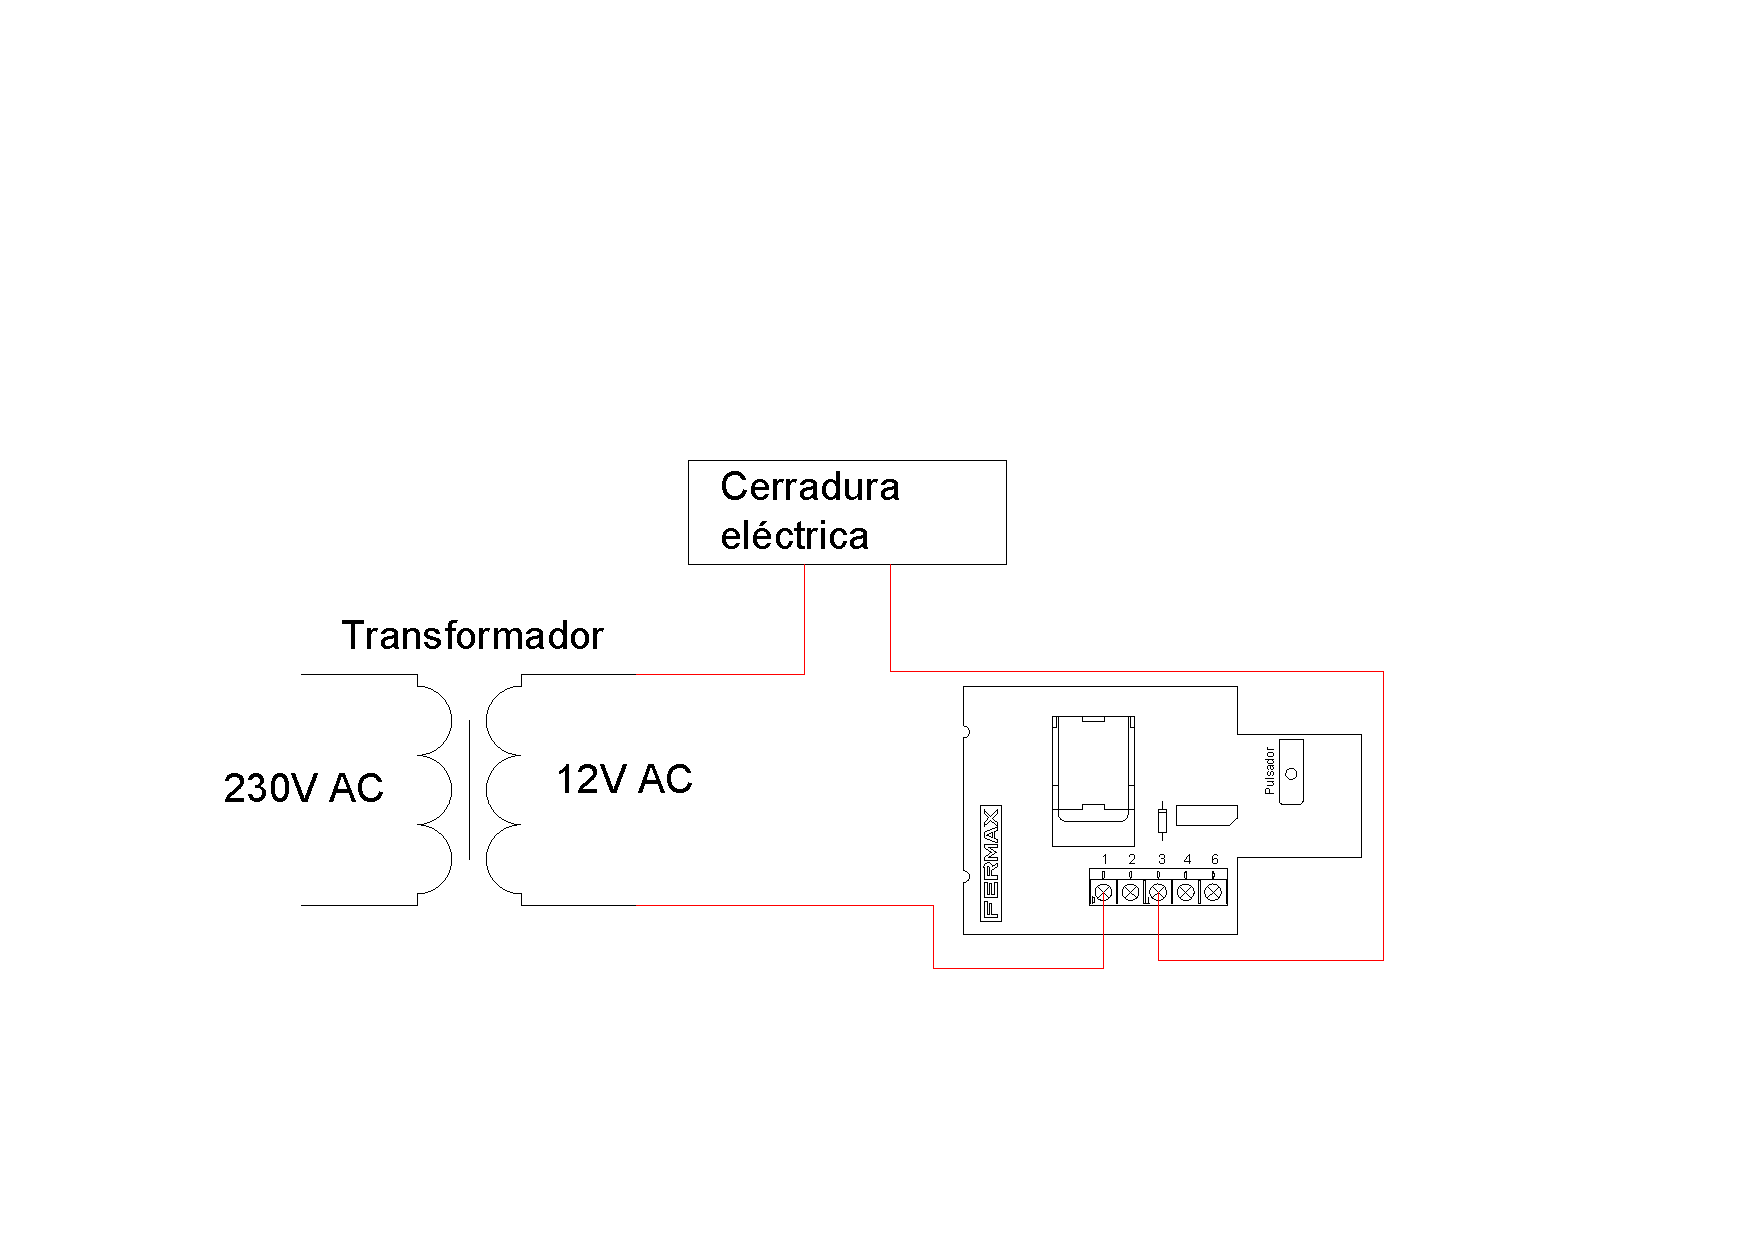
\includegraphics[scale = 0.5]{Conexion-Portero-Cerradura.pdf}
\caption{Conexión de funcionamiento entre el portero automático y la cerradura eléctrica}
\label{fig:conexion-portero-cerradura}
\end{figure}
Como puede observarse en la figura~\ref{fig:conexion-portero-cerradura}, la cerradura eléctrica se activaría siempre que el portero automático permita el paso de corriente. En el caso habitual, el accionamiento del pulsador por parte de cualquier usuario permitiría esta conducción de corriente, sin embargo, en el caso de este trabajo de fin de grado, se debe lograr tal propósito por medio de la activación de una señal de 3V, que es la que la Raspberry Pi Zero W permite emitir a partir de sus puertos programables.

Para llevar a efecto esta tarea será necesario realizar un circuito adicional que permita, siempre que se considere oportuno, el paso de corriente entre los dos bornes del pulsador, haciendo así que el circuito se cierre y se abra cuando se accione la señal emitida por la Raspberry Pi.

Con el fin de resolver este problema, se ha hecho uso de los siguientes elementos:
\begin{itemize}
\item{Relé 5VDC | Modelo: TONGLING JQC-3FF-S-Z}
\item{Conversor de niveles lógicos 3.3/5V | Modelo: Qifei cyt1082}
\item{Raspberry Pi Zero W}
\end{itemize}
En la figura~\ref{fig:conexion-keyhome-completa} se describe el circuito completo que permite realizar la apertura de la cerradura eléctrica por medio de una señal de 3.3V emitida por una Raspberry Pi Zero W:
\begin{figure}[tbp]
\centering
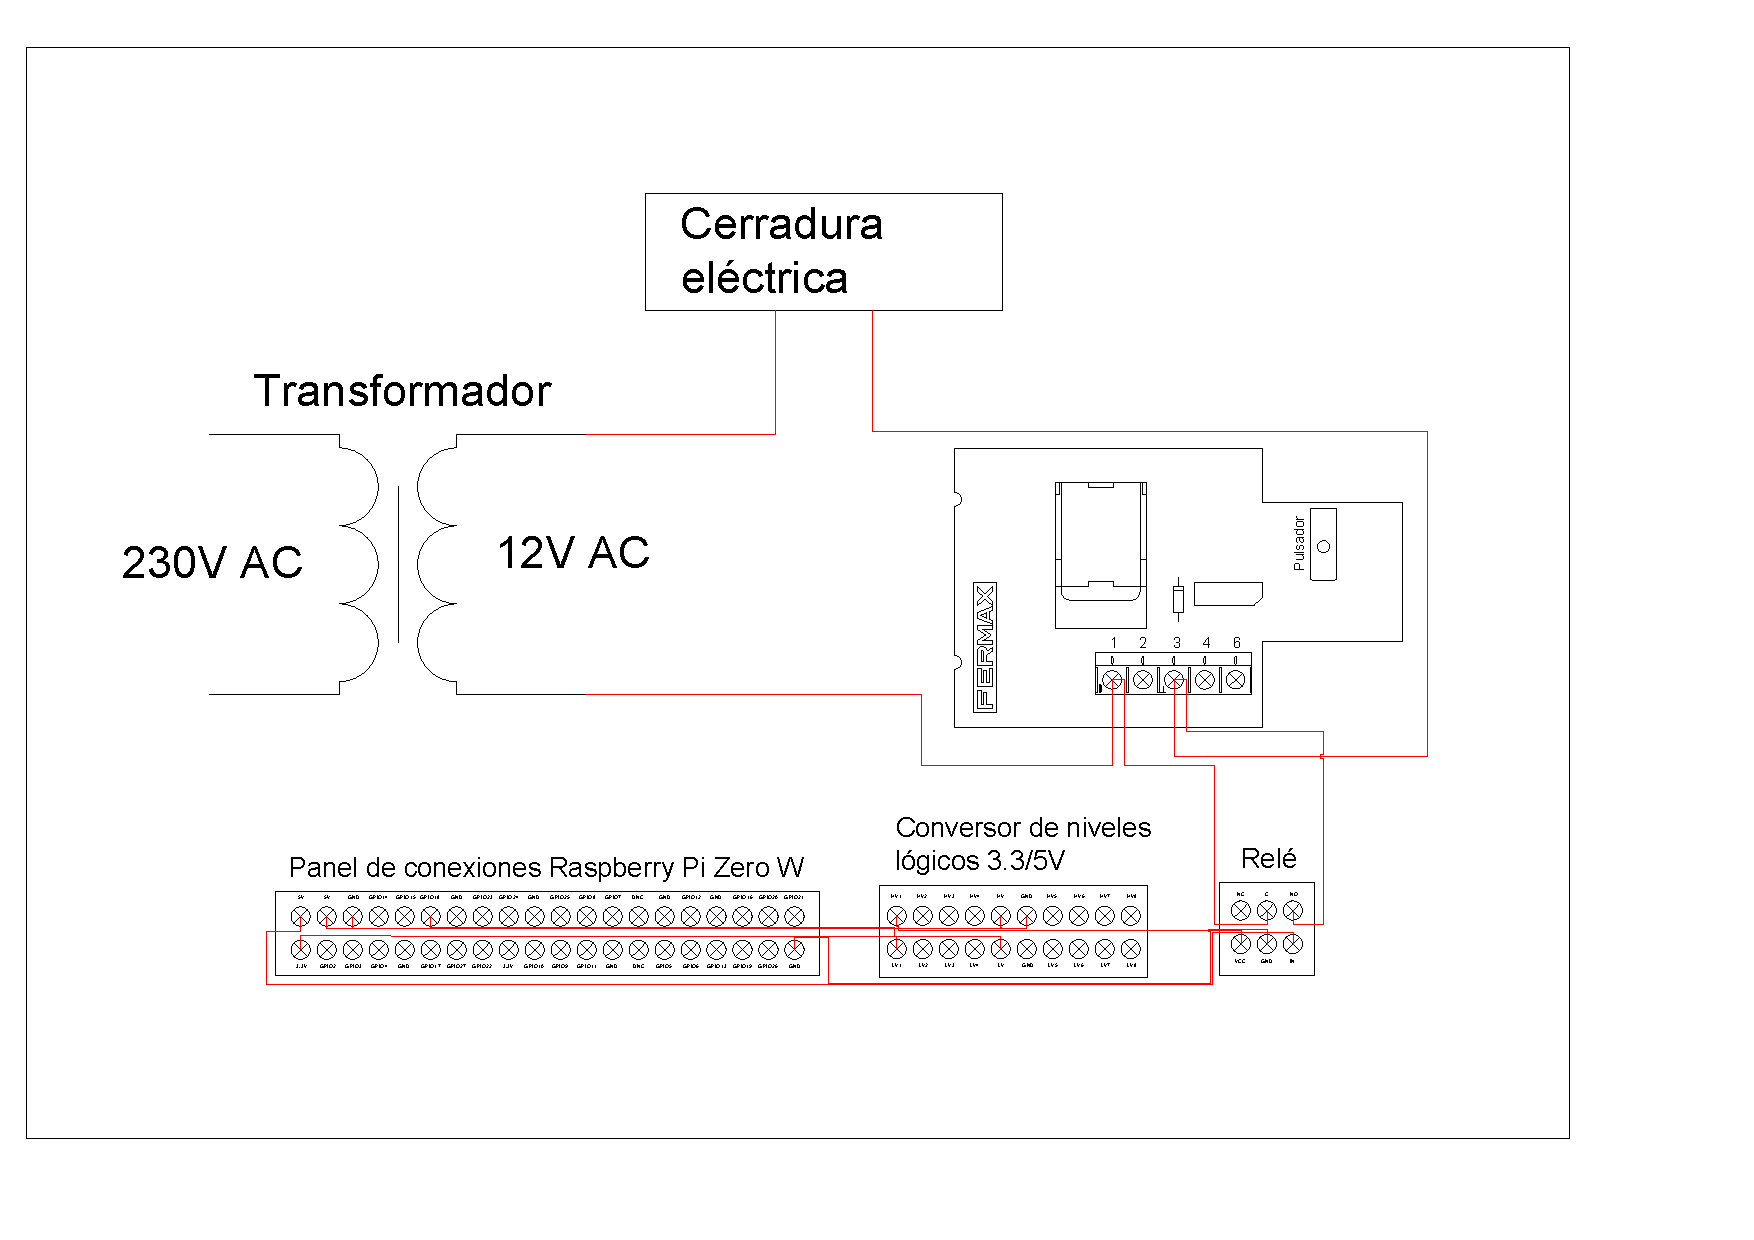
\includegraphics[scale = 0.5]{conexion-keyhome-completa.pdf}
\caption{Conexión de funcionamiento del prototipo completo}
\label{fig:conexion-keyhome-completa}
\end{figure}
Ahora, con el nuevo planteamiento especificado en este circuito, se obtiene el resultado esperado, haciendo que además de poder realizar la apertura de la cerradura por medio de una pulsación física sobre el pulsador del portero automático, pueda hacerse a través de una señal emitida por la Raspberry Pi Zero W con valor de 3V.
Para que se active dicha cerradura eléctrica es necesario que el circuito se cierre sin necesidad de hacer uso del pulsador, y para ello se ha hecho uso de un relé que, al recibir una señal de 5V, permite el paso de corriente entre los terminales 1 y 3 del portero automático.

Como las señales emitidas por la Raspberry Pi son de 5V, no sirven para realizar la activación del señal, por ello se ha empleado un conversor de niveles lógicos que convierte dicha señal de 3V en una de 5V, haciendo así que la señal recibida por el relé permita, de forma correcta, el paso de corriente entre sus terminales.
Con este nuevo diseño, la corriente encuentra dos lugares a través de los cuales puede circular, según se requiera:
\begin{itemize}
\item{A través de los terminales del pulsador cuando este es activado}
\item{A través del relé cuando este recibe una señal de la Raspberry Pi Zero W}
\end{itemize}
Con el fin de poder transportar el prototipo de forma segura y de que las conexiones sean estables, se ha procedido a soldarlas y a fijar cada uno de los elementos con firmeza en una tabla.

\subsection{Diseño de algoritmos y programación}
Una vez que el prototipo ha sido desarrollado y probado con éxito, llega el momento de hacer que las señales se activen en el momento correcto, de manera que todo funcione de forma precisa. Para ello, tal como se ha definido en el apartado de planificación del proyecto, se ha decidido dividir el desarrollo de software en cuatro etapas diferenciadas que, una vez completadas, harán que el prototipo proporcione los resultados esperados. En este apartado se describen los trabajos desarrollados en el orden lógico temporal que fueron realizados.

Lo primero que debe tenerse en cuenta es que la versión de python que viene por defecto en este modelo de Raspberry Pi, es la 2, mientras que la librería ApiTelegramBotAPI, encargada de ejecutar las funciones del bot, funciona con python3, por lo que será necesario instalar esta versión de python\footnote{\url{https://www.altaruru.com/python3-6-en-raspberry-pi/}} en la computadora, de forma previa a la ejecución de los programas previstos.

Antes de llevar a cabo la elaboración de ningún programa, es preciso realizar las configuraciones que permitan trabajar en la Raspberry Pi Zero W con las librerías que se ejecutarán en los archivos de python, de manera que todo funcione y se ejecute de forma correcta. Para llevar a cabo, se hace uso del sistema de gestión de paquetes llamado "pip", el cual permite la instalación de las distintas librerías, necesarias para la ejecución material de este proyecto, de forma sencilla. Para hacer uso de este sistema en la instalación de paquetes para python3, simplemente debe ejecutarse el comando "sudo pip3 install --upgrade pip" en la consola de la Raspberry Pi, y de esta manera se dispondrá de la última versión de este instalador.

Cuando se cuenta con "pip3", la instalación de los paquetes se resume a una ecuación de carácter sencilla, que se ejecutará en la consola de comandos y seguirá siempre la siguiente estructura:

\begin{equation} 
pip3 + install + "Nombre_paquete"
\label{eq:funcionamiento-pip3}
\end{equation}

El primer programa que se pretende definir es aquel que hará que la Raspberry Pi Zero W envíe una señal con el fin de activar la cerradura eléctrica en los momentos que resulten convenientes. A lo largo de este subcapítulo, se irán mostrando y comentando las distintas partes del código que permite cumplir dichas funciones.

\begin{lstlisting}[language=Python,
    caption={Importación de librerias},
    label=src:importacion-librerias
]
import RPi.GPIO as GPIO
import time
GPIO.setmode(GPIO.BCM)
GPIO.setup(18, GPIO.OUT)
import telebot
from telebot import types
import unidecode
import random
from datetime import datetime, date, timedelta
import calendar
\end{lstlisting}

Lo primero que se realiza en el código, tal como puede observarse en el listado 5.1, es importar cada una de las librerías que serán necesarias para su desarrollo. Estas librerías están destinadas a trabajos diversos, como puede ser implementar la funcionalidad del envío de señales por medio de la Raspberry Pi, trabajar con la aplicación de Telegram, hacer uso de números aleatorios u operar con fechas. Todas estas librerías desarrollarán funciones específicas a lo largo del código que puede observarse en el listado 5.2.
\begin{lstlisting}[language=Python,
    caption={Inicializar variables},
    label=src:inicializar-variables
]
fechasiniciales=[]
fechasfinales=[]
contrasenas=[]
fechainiciousuario=[]
fechafinalusuario=[]
fechas = str(datetime.now())
ano = int(fechas[0:4])
mes = int(fechas[5:7])
dia = int(fechas[8:10])
usuariosactivos=[]
administradores=[]
listanegra=[]
paso1=False
paso2=False
paso3=False
paso0=False
intentos = 0 
contador_intentos_erroneos = []
numreserva = ""
bot = telebot.TeleBot('TOKEN')
\end{lstlisting}
En el listado 5.2 se procede a inicializar algunas de las variables con las que se irán trabajando a lo largo de este programa. También se incluye en esta parte el Token ofrecido por la plataforma de Telegram, el cual permite conectar con el bot de forma segura.
\begin{lstlisting}[language=Python,
    caption={Función que convierte el string de reservas en un vector},
    label=src:string-a-vector
]
def convierteavector(texto):
    if len(texto) > 0:
        texto = texto.replace("'","")
        texto = texto.replace("[","")
        texto = texto.replace("]","")
        texto = texto.replace(" ","")
        vector = texto.split(',')
        return vector
\end{lstlisting}
La función que se muestra en el listado 5.4 servirá para convertir una cadena de texto común en un vector, que como se verá más adelante, resultará de utilidad para el correcto funcionamiento del programa. Las reservas que se irán recibiendo, tanto las creadas por parte del administrador como las que se reciban de las compañías de alquiler vacacional, se irán almacenando en un documento de extensión .txt que registrará el número de reserva y la fecha de entrada. Estos datos estarán almacenados en un vector que será convertido a texto con el fin de integrarse en el documento .txt de forma que, aunque la Raspberry Pi Zero W se apague, la información se pueda recuperar de forma segura.
\begin{lstlisting}[language=Python,
    caption={Función que verifica si una petición es posterior a la fecha inicial de la reserva},
    label=src:comprueba-fecha-inicial
]
def comprobarfecha(fechainic):
    fechas = str(datetime.now())
    ano = int(fechas[0:4])
    mes = int(fechas[5:7])
    dia = int(fechas[8:10])
    hora = int(fechas[11:13])
    anop = int(fechainic[0:4])
    mesp = int(fechainic[5:7])
    diap = int(fechainic[8:10])
    if anop == ano and mesp == mes and diap == dia:
        if hora >= 15:
            return True
        else:
            return False   
    elif ano > anop:
        return True
    elif ano == anop and mes > mesp:
        return True
    elif ano == anop and mes == mesp and dia >= diap:
        return True
    else:
        return False
\end{lstlisting}
En el listado 5.4 se muestra una función que servirá al programa para verificar si la persona que trata de acceder a la vivienda lo hace en un marco temporal posterior a la fecha inicial de su reserva. En caso de que se cumpla, devolverá un booleano verdadero y, en caso de que no se cumpla, devolverá un booleano falso. Puede observarse que la hora mínima que se ha puesto para acceder a la vivienda son las 15pm. Esta decisión se ha tomado ya que parece ser el horario habitual en la mayoría de destinos hoteleros, sin embargo este es un factor que puede ser alterado por el propietario siempre que lo considere oportuno.
\begin{lstlisting}[language=Python,
    caption={Función que verifica si una petición es anterior a la fecha final de reserva},
    label=src:comprueba-fecha-final
]
def comprobarfechamaxima(fechafin):
    fechas = str(datetime.now())
    ano = int(fechas[0:4])
    mes = int(fechas[5:7])
    dia = int(fechas[8:10])
    hora = int(fechas[11:13])
    anop = int(fechafin[0:4])
    mesp = int(fechafin[5:7])
    diap = int(fechafin[8:10])
    if anop == ano and mesp == mes and diap == dia:
        if hora < 12:
            return True
        else:
            return False
    elif anop > ano:
        return True
    elif anop == ano and mesp > mes:
        return True
    elif anop == ano and mesp == mes and diap > dia:
        return True
    else:
        return False
\end{lstlisting}
Al igual que se debe conocer si una petición de acceso se está realizando de forma posterior al momento inicial de la reserva, se debe saber también si esta se realiza de forma anterior a la fecha final de la misma. Para ello, se crea la función definida en el listado 5.5, la cual determina si dicha condición se cumple devolviendo un booleano verdadero. La hora máxima de entrada en el último día de reserva es, en este caso, las 12 del medio día.
\begin{lstlisting}[language=Python,
    caption={Función que verifica si se ha introducido una fecha de forma correcta},
    label=src:comprueba-formato-fecha
]
def comprobarfechaintroducida(fechapalabra):
    numeros=["0","1","2","3","4","5","6","7","8","9"]
    if len(fechapalabra)==10:
        if fechapalabra[0] in numeros and fechapalabra[1] in numeros and fechapalabra[2] in numeros and fechapalabra[3] in numeros and fechapalabra[5] in numeros and fechapalabra[6] in numeros and fechapalabra[8] in numeros and fechapalabra[9] in numeros:
            return True
        else:
            return False
    else:
        return False
\end{lstlisting}
Una de las funcionalidades que tendrá el programa completo, será la de permitir, a través de la aplicación de Telegram, que el administrador de la vivienda pueda crear nuevas reservas siempre que lo desee. Para ello será necesario que introduzca las fechas correspondientes a dicha reserva. La función descrita en el listado 5.6 se encarga de verificar que la fecha se ha introducido de forma correcta según se lo exige el propio bot de Telegram. Su comportamiento, al igual que en las funciones anteriores, será booleano, ofreciendo una respuesta verdadera en caso de que se cumpla dicha condición, y una falsa en el caso contrario.
\begin{lstlisting}[language=Python,
    caption={Función que activa una señal de voltaje desde la Raspberry Pi},
    label=src:activar-senal
]
def blink():
        
        GPIO.setmode(GPIO.BCM)
        iteracion = True
        while iteracion == True:
                GPIO.output(18, True)
                time.sleep(5)
                break
        GPIO.output(18, False)
\end{lstlisting}
Por medio de la función que puede observarse en el listado 5.7 se activa la señal que, en conjunto con el circuito definido en la sección anterior, hace que se active la cerradura eléctrica, permitiendo así el acceso de los usuarios a la vivienda. Se ha utilizado el puerto GPIO18 y se ha dado un tiempo de activación de 5 segundos, de manera que el usuario tenga un espacio temporal suficientemente amplío para abrir la puerta después de haber hecho la petición a través de su aplicación de Telegram.
\begin{lstlisting}[language=Python,
    caption={Primer contacto con el bot de Telegram},
    label=src:primer-contacto-con-bot
]
@bot.message_handler(commands=["start","comenzar"])
def send_welcome(message):
    
    chatid = message.chat.id
    nombreUsuario = message.chat.first_name
    nombreUsuario = unidecode.unidecode(nombreUsuario)
    saludo = "Hola {nombre}, bienvenido a KeyHome! Ya estás un paso más cerca de acceder a tu vivienda! Por favor, necesito que me indiques el número de tu reserva"
    bot.send_message(chatid, saludo.format(nombre=nombreUsuario))
\end{lstlisting}
Cuando un usuario accede por primera vez a un bot de Telegram, el bot le ofrece la opción de iniciar la conversación con la palabra "start". El primer contacto con el bot es un buen momento para realizar a los usuarios las instrucciones que deben llevar a cabo para guiarles de forma correcta. En el código del listado 5.8 se recoge el nombre  y una identificación única de Telegram de cada usuario. Posteriormente se crea el mensaje de saludo y por último se le envía.
\begin{lstlisting}[language=Python,
    caption={Recepción de mensajes por parte de los usuarios},
    label=src:recepcion-mensajes-usuarios
]
@bot.message_handler(func=lambda message: True)
def echo_all(message):
    chatid = message.chat.id
    chatod = str(chatid)
    a=message.text
    global paso1, paso2, paso3, paso0, fechaentrada, fechasalida, nuevapass, intentos, contador_intentos_erroneos, listanegra, fechainiciousuario, fechafinalusuario, numreserva
    if chatod in listanegra:
        bot.send_message(chatod, "Lo siento, has agotado todos los intentos posibles")
\end{lstlisting}
En este momento se procede a atender los mensajes de los usuarios diferentes al saludo inicial. Durante el desarrollo de este proceso se ha hecho uso, como puede observarse en el listado 5.9, de diferentes variables globales que se irán viendo a lo largo del código que se muestra a continuación.
En este primer contacto con las peticiones del usuario, se ha procedido a convertir su id numérica en una cadena de texto con la que poder trabajar, y también se ha recogido el mensaje recibido.
Puede observarse, en las últimas líneas, que el primer filtro que pasa el usuario es el de no estar en un vector llamado "listanegra". Este vector tiene la misión recoger aquellos usuarios que han tenido más de 50 intentos erróneos tratando de acceder a la vivienda. Esta medida se toma con carácter preventivo ante posibles ataques, de manera que ningún ordenador pueda dedicarse a enviar números a gran escala con el fin de averiguar los números de reserva activos.
Una vez pasado el filtro de aquellos usuarios que forman parte del vector "listanegra", caben tres posibilidades: que el usuario sea un administrador, un cliente final, o que todavía no esté registrado de ninguna manera.
\begin{lstlisting}[language=Python,
    caption={Panel de administrador},
    label=src:panel-de-administrador
]
    else:
        if a == password_admin:
            mensajetipo="Ahora eres administrador de esta vivienda"
            markup=types.ReplyKeyboardMarkup()
            markup.row('Nueva reserva','Abrir puerta')
            markup.row('Dejar de ser administrador','Ver reservas activas')
            bot.send_message(chatod, mensajetipo, None, None, markup)
            if chatod not in administradores:            
                administradores.append(chatod)
\end{lstlisting}
La primera parte de este código, tal como puede observarse en el listado 5.10, consiste en otorgar los permisos de administrador a aquellos usuarios que indiquen de forma correcta la contraseña de administradores.
Una vez que el usuario recibe estos permisos especiales, se le ofrece un panel de administrador con cuatro opciones: Dejar de ser administrador, ver reservas activas, crear una nueva reserva y abrir la puerta.

\begin{lstlisting}[language=Python,
    caption={Crear nueva reserva},
    label=src:crear-nueva-reserva
]
        elif chatod in administradores:
            if a == "Nueva reserva":
                bot.send_message(chatod, "Por favor, indique el número de la reserva")
                paso0 = True
            elif paso0 == True: 
                numreserva = a
                bot.send_message(chatod, "Por favor, indique la fecha inicial para los clientes:")
                bot.send_message(chatod, "Ejemplo: 2019-06-25")
                paso1=True
                paso2 = False
                paso3 = False
                paso0 = False
            elif paso1 == True:
                if paso2 == True or paso1 == True or paso3 == True:
                    paso1 = False
                    paso2 = False
                    paso3 = False
                comprobar=comprobarfechaintroducida(a)
                if comprobar == True:
                    bot.send_message(chatod, "Ahora introduzca la fecha final:")
                    bot.send_message(chatod, "Ejemplo: 2019-06-28")
                    fechaentrada=a
                    paso2=True
                else:
                    markup=types.ReplyKeyboardMarkup()
                    markup.row('Nueva reserva','Abrir puerta')
                    markup.row('Dejar de ser administrador','Ver reservas activas')
                    bot.send_message(chatod, "La fecha introducida no es correcta, por favor, vuelve a comenzar", None, None, markup)
                    paso1=False
            elif paso2==True:
                if paso2 == True or paso1 == True or paso3 == True:
                    paso1 = False
                    paso2 = False
                    paso3 = False
                comprobar=comprobarfechaintroducida(a)
                if comprobar == True:
                    nuevapass=numreserva
                    fechasalida=a
                    bot.send_message(chatod, "Genial, se ha creado una nueva entrada. Los clientes podrán acceder a la vivienda desde la fecha "+fechaentrada+" hasta la fecha "+fechasalida+". \nPara acceder, sus clientes deberán introducir únicamente su número de reserva")
                    bot.send_message(chatod, nuevapass)
                    fechasiniciales.append(fechaentrada)
                    fechasfinales.append(fechasalida)
                    contrasenas.append(nuevapass)
                    f = open ('reservas.txt','r')
                    texto = f.read()
                    f.close()
                    vector = []
                    if len(texto) > 0:
                        vector = convierteavector(texto)
                    fechaentrada = fechaentrada.split("-")
                    vector.append(str(fechaentrada[0]))
                    vector.append(str(fechaentrada[1]))
                    vector.append(str(fechaentrada[2]))
                    vector.append(nuevapass)
                    f = open ('reservas.txt','w')
                    f.write(str(vector))
                    f.close()                    
                else:
                    bot.send_message(chatod, "La fecha introducida no es correcta, por favor, vuelve a empezar")
                    paso2=False
\end{lstlisting}
Cuando un usuario es reconocido como administrador, puede crear reservas. De la habilitación de esta funcionalidad se encarga el código del listado 5.11, por medio del cual, se realiza esta operación. El algoritmo del proceso que se observa en la figura~\ref{fig:proceso-nueva-reserva} refleja con claridad como funciona este proceso.

\begin{figure}[tbp]
\centering
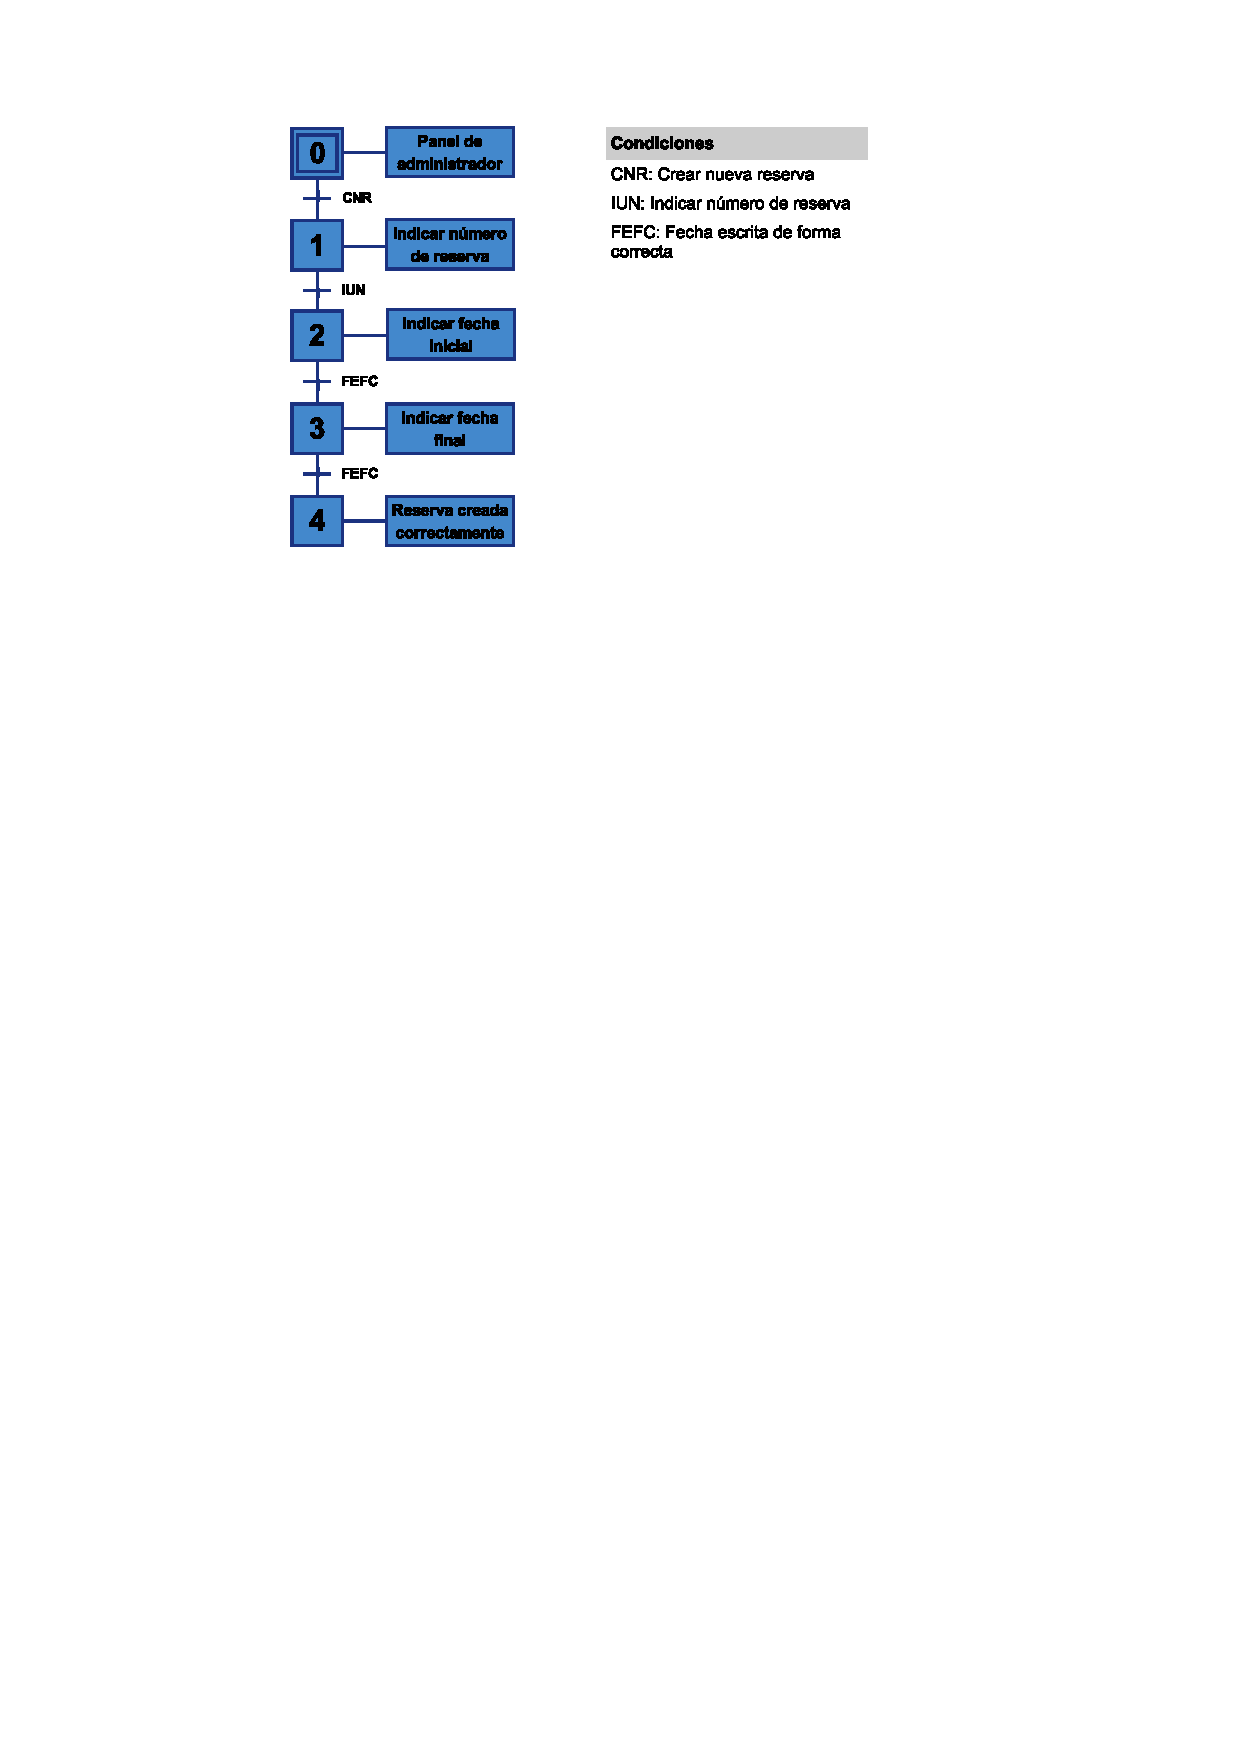
\includegraphics[scale=1]{fig/Grafcet_creacion_nueva_reserva.pdf}
\caption{Proceso de creación de una nueva reserva}
\label{fig:proceso-nueva-reserva}
\end{figure}

En dicho proceso puede observarse como el bot dirige al administrador durante la creación de una nueva reserva, permitiendo que esta se configure solo cuando se cumplen las condiciones necesarias que han sido definidas.
La primera condición debe ser que el administrador elija la opción de "Crear una nueva reserva", en cuyo caso, lo primero que hará el bot será pedirle un número de reserva. Este número de reserva será el que tendrá que usar aquella persona a la que este destinada la reserva para identificarse ante el bot y poder acceder a la vivienda. El número de reserva podrá estar compuesto por letras, números y otro tipo de caracteres.
Una vez introducido el número de reserva, el bot pedirá al administrador que le indique la fecha inicial. Para poder continuar a partir de este paso, es imprescindible que la fecha se introduzca en el orden que indica el bot (YYYY/MM/DD). En caso de que no se introduzca de esta manera, el bot no permitirá continuar con el proceso.
Habiendo indicado el número de reserva y la fecha inicial, solo quedará indicar la fecha final (con la misma condición que en el caso de la inicial) y el bot habrá dado por concluido el proceso de reserva.
Una vez que se ha indicado la fecha final, el archivo python almacena en el documento que almacena las reservas (reservas.txt), las variables de fecha y número de reserva.
El archivo mencionado "reservas.txt" será el encargado de ir almacenando cada una de las reservas creadas por parte del usuario, las cuales permanecerán a salvo a pesar de una interrupción en el funcionamiento de la Raspberry Pi.
Una vez que el proceso de reserva está listo, puede procederse a habilitar al bot para realizar la función de abrir la cerradura desde el panel de administrador.
\begin{lstlisting}[language=Python,
    caption={Apertura de puertas desde el panel de administración},
    label=src:apertura-puertas-panel-administrador
]
            elif a == "Abrir puerta":
                if paso2 == True or paso1 == True or paso3 == True:
                    paso1 = False
                    paso2 = False
                    paso3 = False
                bot.send_message(chatod, "Abriendo puerta...")
                blink()
\end{lstlisting}
El código que se aprecia en el listado 5.12 es el encargado de permitir el acceso a la vivienda por parte del administrador siempre que lo desee. Puede observarse que, para ello, se hace uso de la activación de la señal por medio de la función blink, explicada con anterioridad en el listado 5.7.
También se destaca como se desactivan todos los pasos correspondientes al proceso de reserva. Esto se realiza con el fin de que, si en mitad de una creación de reserva, el administrador decide abrir la puerta, el programa abriría pero se quedaría en el punto que estaba en esa función paralela, provocando errores en el futuro. Llevando a cabo esta acción se evita este error y se reinician desde el principio todas estas variables.

\begin{figure}[tbp]
\centering
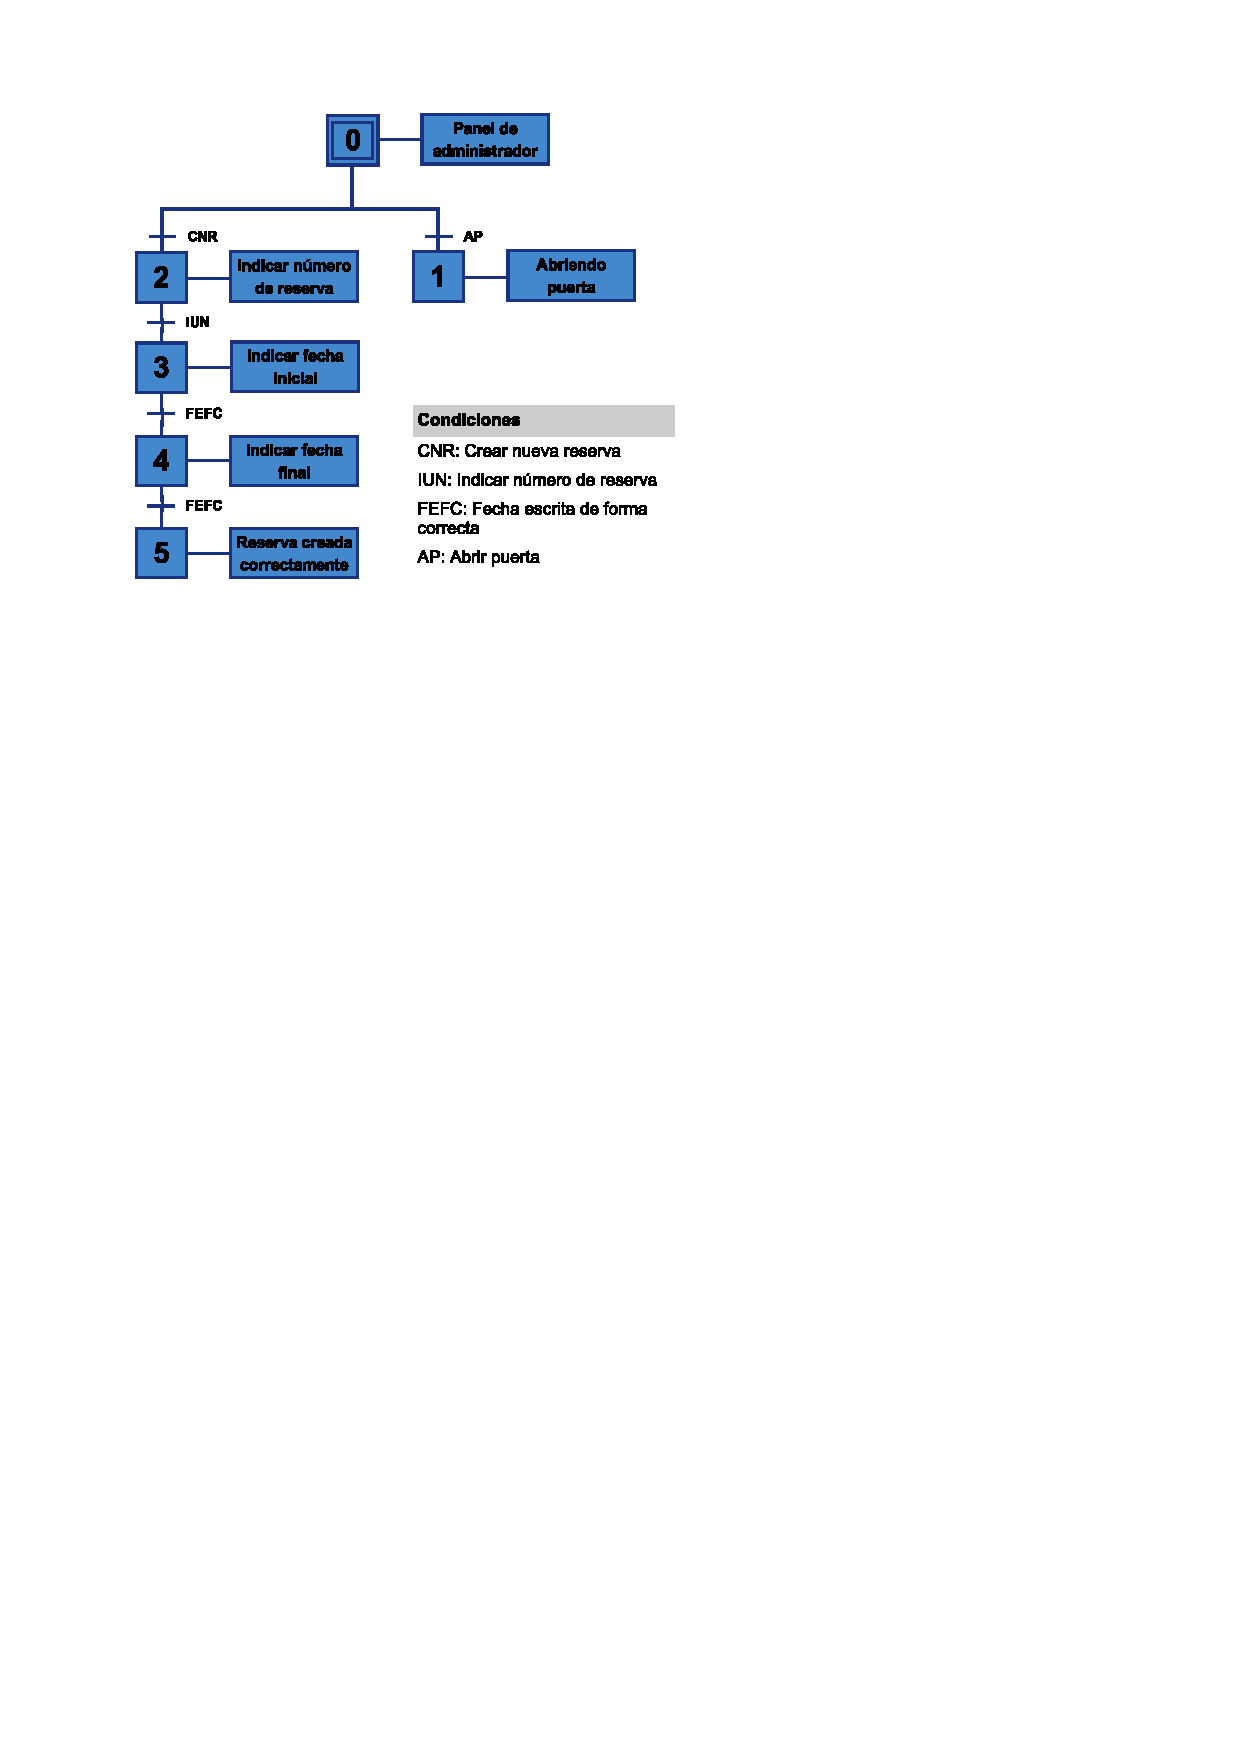
\includegraphics[scale=1]{fig/Grafcet_reserva_y_apertura.pdf}
\caption{Panel de administrador que permite crear reservas y realizar la apertura}
\label{fig:reserva-y-apertura}
\end{figure}

La siguiente opción que ha sido incluida en el panel de administrador es la de ofrecer la posibilidad de dejar de ser administrador. Esta opción puede llevarse a cabo por diferentes razones, como puede ser un administrador temporal (mientras el administrador principal está de vacaciones), para que el administrador principal pruebe el modo usuario, etc. Para conseguir que el bot desarrolle dicha opción, se ha incluido el código que se refleja en el listado 5.13:
\begin{lstlisting}[language=Python,
    caption={Dejar de ser administrador},
    label=src:dejar-de-ser-administrador
]
            elif a == "Dejar de ser administrador":
                if paso2 == True or paso1 == True or paso3 == True:
                    paso1 = False
                    paso2 = False
                    paso3 = False
                administradores.remove(chatod)
                bot.send_message(chatod, "Ya no tienes permisos de administrador")
\end{lstlisting}
En el extracto de código del listado 5.13 puede observarse, al igual que en casos anteriores, como antes de eliminar al usuario de administrador se procede a reinicializar todas las variables del proceso de reserva. Esto se hace con la intención de que no se quede ningún proceso a medias y que, cuando otro administrador trabaje en el bot, no se encuentre ninguna sorpresa.
Para eliminar al usuario como administrador de la propiedad, tan solo ha sido necesario eliminar su número de identificación del vector donde se almacenan los administradores. En la figura~\ref{fig:reserva-apertura-y-dejar-administracion} se muestra el algoritmo que describe el comportamiento del bot tras esta última actualización.
\begin{figure}[tbp]
\centering
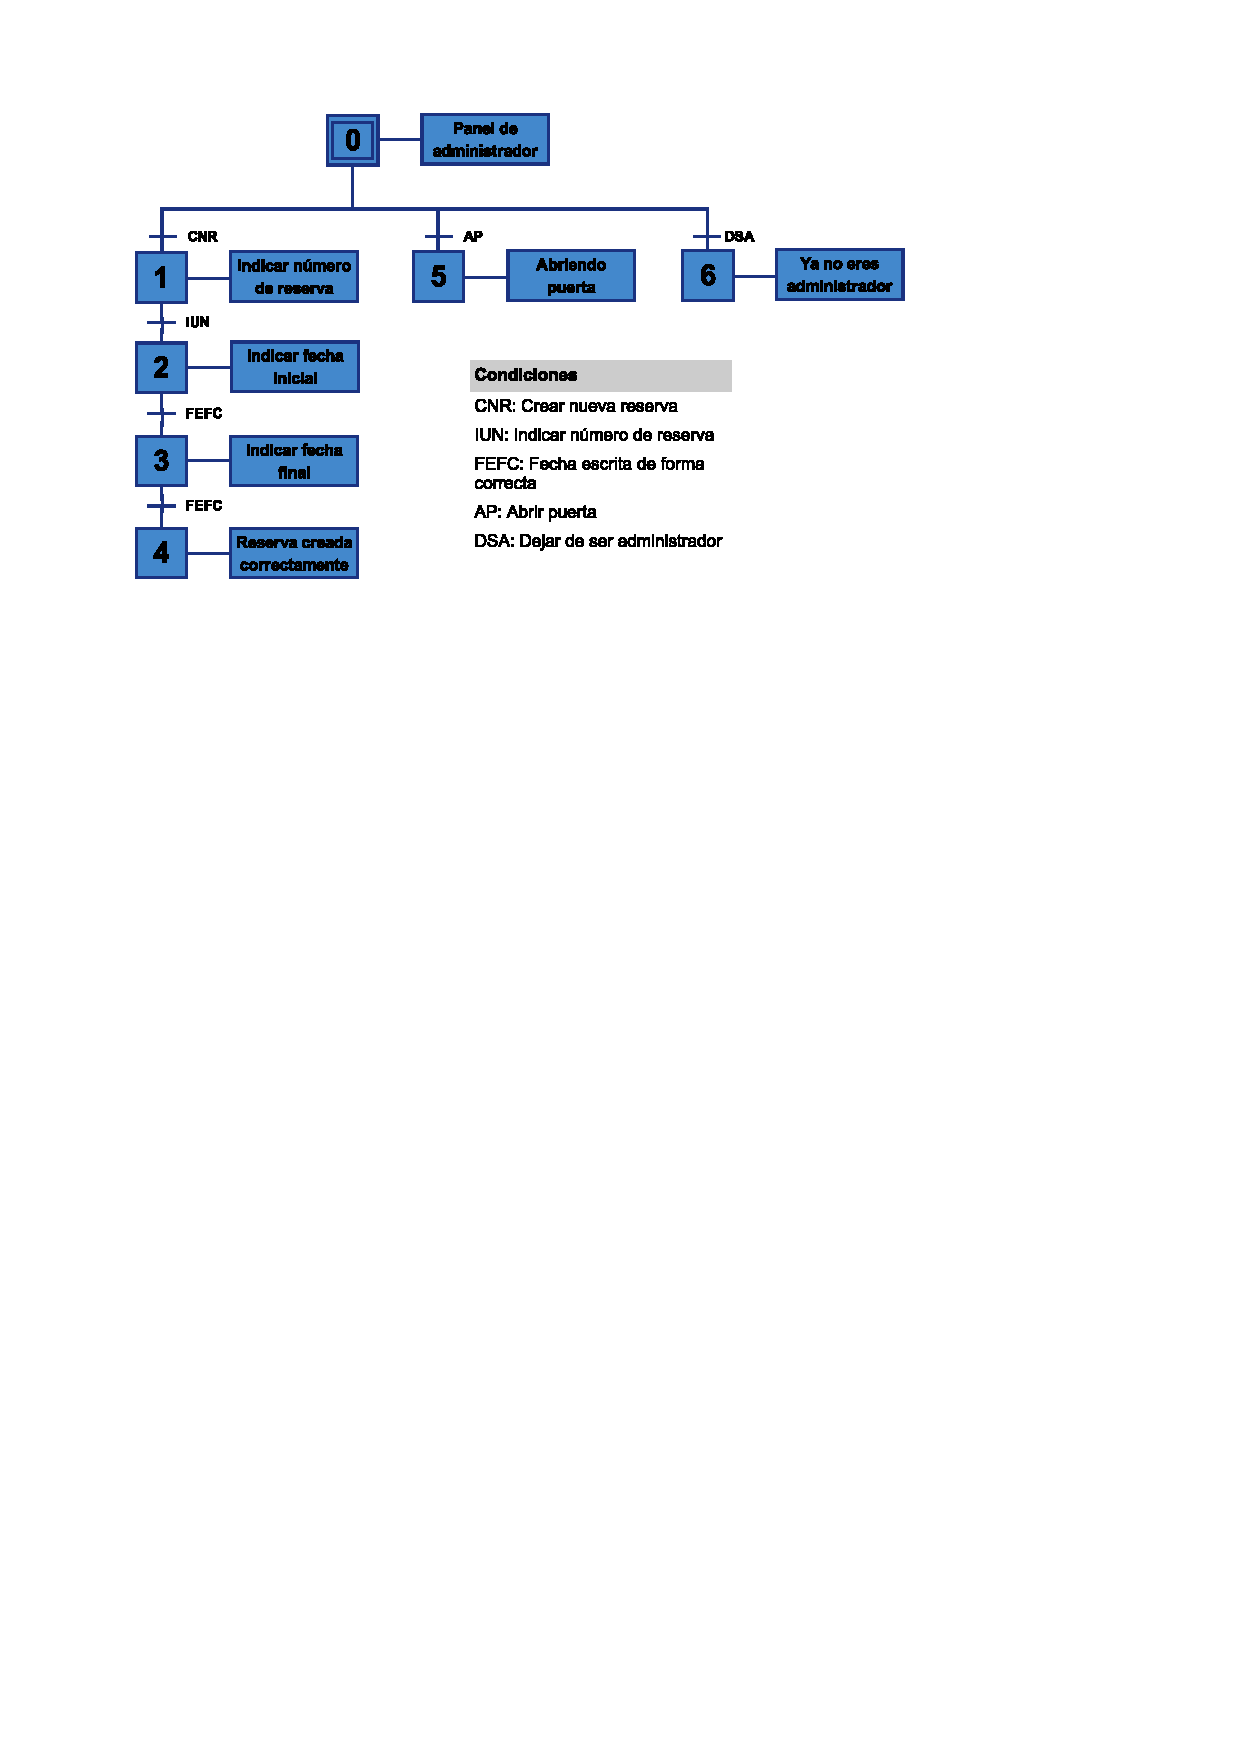
\includegraphics[scale=1]{fig/Grafcet_reserva_apertura_y_dejar_administracion.pdf}
\caption{Panel de administrador que permite crear reservas, realizar aperturas y dejar de ser administrador}
\label{fig:reserva-apertura-y-dejar-administracion}
\end{figure}
Atendiendo a los criterios que fueron definidos en el apartado de planificación del presente proyecto, solo faltaría añadir al panel de administrador la posibilidad de visualizar y/o modificar las reservas activas. El código que se muestra en el listado 5.14 es el encargado de llevar a cabo dicha tarea:
\begin{lstlisting}[language=Python,
    caption={Consulta y modificación de reservas},
    label=src:consulta-y-modificacion-de-reservas
]
                if paso2 == True or paso1 == True or paso3 == True:
                    paso1 = False
                    paso2 = False 
                reservas = ""
                tam = int(len(contrasenas))
                paso3 = True
                f = open ('reservas.txt','r')
                texto = f.read()
                f.close()
                vector = []
                if len(texto) > 0:
                    vector = convierteavector(texto)
                if len(vector)>0:
                    i = 0
                    while i < (len(vector)/4):
                        j=i+1
                        reservas = reservas + (""+str(j)+". Reserva para el día "+str(vector[i*4+2])+"-"+str(vector[i*4+1])+"-"+str(vector[i*4])+" con número de reserva: "+str(vector[i*4+3])+"\n")
                        i+=1
                    bot.send_message(chatod, reservas)
                    bot.send_message(chatod, "Si quieres eliminar alguna reserva, simplemente escribe el número que deseas eliminar")
                else:
                    bot.send_message(chatod, "No hay reservas activas")
            elif paso3 == True:
                paso3 == False
                f = open ('reservas.txt','r')
                texto = f.read()
                f.close()
                comprueba = compruebaentero(a)
                vector = convierteavector(texto)
                cantidad = (len(texto)/4)
                if comprueba == True:
                    if cantidad >= int(a):
                        a = int(a)
                        nr = a
                        a = (a - 1)*4
                        for i in range(4):
                            vector.pop(a)
                        f = open ('reservas.txt','w')
                        f.write(str(vector))
                        f.close()                                                 
                        bot.send_message(chatod, "Se ha borrado la reserva "+str(nr))
                    else:
                        bot.send_message(chatod, "El número no corresponde a ninguna reserva")
                else:
                    bot.send_message(chatod, "Lo siento, pero no entiendo el mensaje")
            else:
                bot.send_message(chatod, "No entiendo el mensaje")
\end{lstlisting}

Las líneas descritas en el listado 5.14 muestran el proceso que sigue el programa a la hora de realizar la consulta de reservas. Para realizar esta tarea de forma correcta, se deben tener en cuenta las dos opciones posibles en la consulta, donde la primera sería que haya reservas y en ese caso mostrarlas, y la segunda consistiría en que no haya reservas, y en ese caso transmitir esa información al administrador.

Solo en el caso de que haya reservas activas, se notificará al usuario la cantidad total de las mismas y se le ofrecerá la posibilidad de eliminar aquellas que desee, simplemente introduciendo el número correspondiente a dicha reserva.

El diagrama que se observa en la figura~\ref{fig:panel-administrador-completo} tiene por objeto mostrar, de forma más gráfica, el funcionamiento del panel de administrador que se ha dispuesto en el bot de Telegram.

\begin{figure}[tbp]
\centering
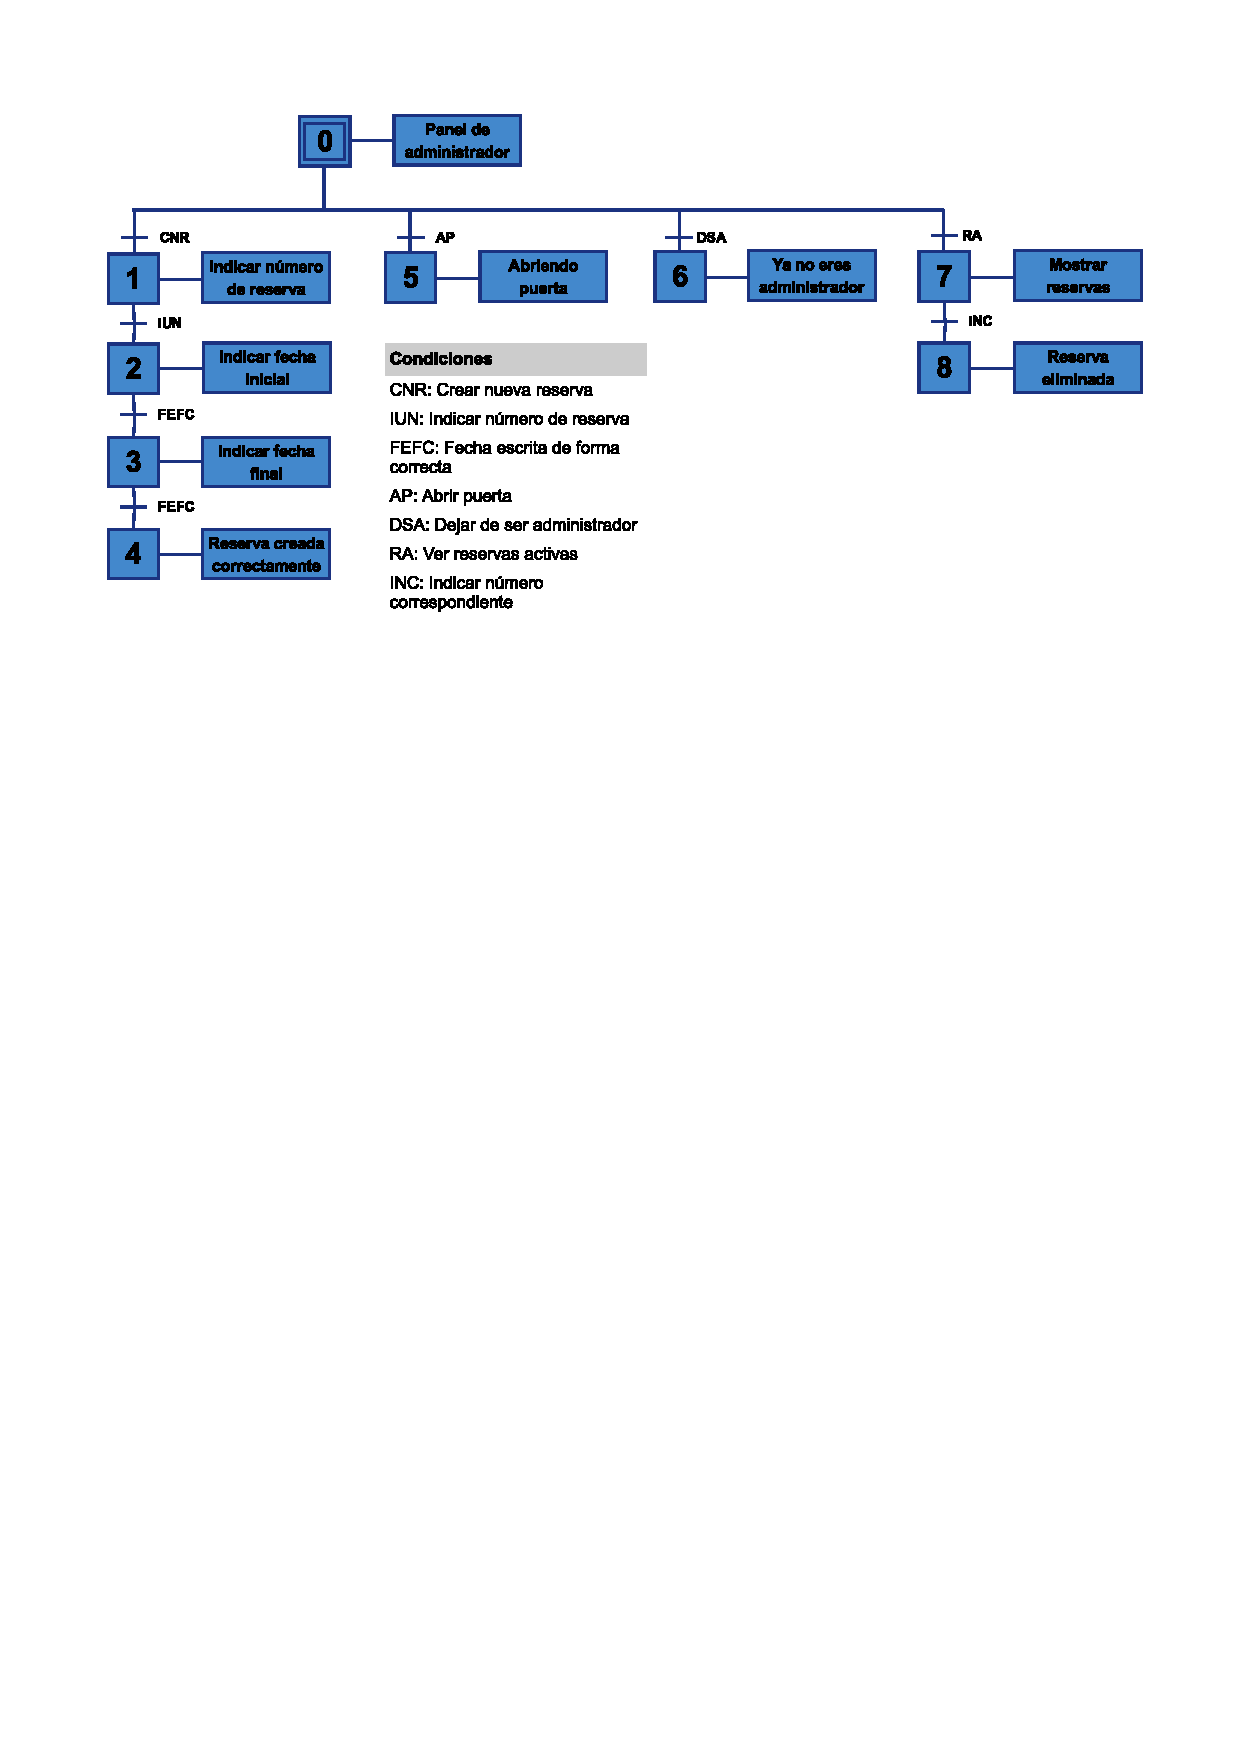
\includegraphics[scale=0.8]{fig/Panel_administrador_completo.pdf}
\caption{Panel de administrador completo}
\label{fig:panel-administrador-completo}
\end{figure}

Habiendo finalizado el proceso de consulta y modificación de reservas, se dan por completados todas las características previas que se definieron anteriormente sobre las opciones del administrador. Es momento, por tanto, de realizar la programación necesaria para autorizar la apertura de puertas a los usuarios finales.
Esta parte del código, a pesar de que se plantea de forma más sencilla que la anterior, debe tener en cuenta también diferentes factores y posibilidades distintas. Un usuario puede hacer una petición de apertura, pero para ello, se debe conocer primero si este usuario esta autorizado o no a llevar a cabo tal acción. Por ello, la primera parte de este código tendrá por objeto identificar si este usuario está activo, y en caso de que lo esté, comprobará si todavía está dentro de fecha para poder realizar aperturas.

En el caso de que el tiempo de estancia del huésped ya haya pasado, será eliminado de forma inmediata del vector de usuarios activos y se le anulará la posibilidad de realizar aperturas.
El código que se muestra en el listado 5.15 tiene por objeto hacer cumplir estas condiciones.

\begin{lstlisting}[language=Python,
    caption={Comprobar huéspedes activos},
    label=src:comprobar-huespedes-activos
]
        else:
            if paso3 == True or paso2 == True or paso1 == True:
                paso3 = False
                paso2 = False
                paso1 = False
            if chatod in usuariosactivos:
                posicion = int(usuariosactivos.index(chatod))
                fechamax = fechafinalusuario[posicion]
                comprobar = comprobarfechamaxima(fechamax)
                if comprobar == False:
                    usuariosactivos.remove(chatod)
                if chatod in usuariosactivos:                    
                    if a == "Abrir" or a == "abrir" or a == "Abrir puerta":            
                        bot.send_message(chatod, "Abriendo puerta...")
                        blink()                        
                    else:
                        bot.send_message(chatod, "Recuerda que para abrir solo necesitas escribir la palabra Abrir o pulsar el boton")
\end{lstlisting}

Puede observarse además, que el usuario tiene tres opciones distintas para realizar la apertura, escribiendo "abrir", "Abrir" o "Abrir puerta", y en caso de que no coincida con ninguna, se le enviarán instrucciones de como realizar la apertura.
Ahora debe tratarse la segunda posibilidad, que sería aquella en la que el usuario todavía no se ha registrado como huésped, y por tanto, debe identificarse para que el bot pueda definir correctamente si este tiene o no permisos de apertura.

Para realizar esta operación de forma correcta, será necesario consultar las reservas activas a través del documento reservas.txt, y en caso de que el número de reserva indicado por el usuario sea correcto, se deberá verificar que se encuentra dentro de plazo. Esta operación se realiza a través del código que se observa en el listado 5.16.
\begin{lstlisting}[language=Python,
    caption={Registrar nuevo huesped},
    label=src:registrar-nuevo-huesped
]
            else:
                f = open ('reservas.txt','r')
                texto = f.read()
                f.close()
                vector = convierteavector(texto)
                if a in vector:
                        posicion=vector.index(a)
                        fechainic=(""+vector[posicion-3]+"-"+vector[posicion-2]+"-"+vector[posicion-1])
                        fechafin = datetime.strptime(fechainic, '%Y-%m-%d')
                        fechafin = fechafin + timedelta(days=1)
                        fechafin = str(fechafin)
                        verificafechainic=comprobarfecha(fechainic)
                        verificafechafin=comprobarfechamaxima(fechafin)
                        if verificafechainic==True and verificafechafin==True:                            
                            mensajetipo="Enhorabuena! Ya puedes acceder a tu vivienda pulsando o escribiendo Abrir. Espero que tengas una gran estancia"
                            markup=types.ReplyKeyboardMarkup()
                            markup.add('Abrir puerta')
                            usuariosactivos.append(chatod)
                            fechafinalusuario.append(chatod)
                            bot.send_message(chatod, mensajetipo, None, None, markup)     
                        else:
                            bot.send_message(chatod, "Su reserva está fuera de fecha, recuerda que esta reserva corresponde al periodo del "+fechainic+"a las 12:00 hasta "+fechafin+" a las 15:00")
\end{lstlisting}
Con esto quedaría definido el papel del usuario final en este programa, tanto en caso de estar registrado, como en el de necesitar su registro en la plataforma.
No obstante, para evitar que, de forma malintencionada, se intente desbloquear el acceso a la vivienda introduciendo miles de números distintos por medio de un ordenador, se ha limitado la posibilidad de equivocarse con el número de reserva a 50 veces. En el código que se muestra a continuación, se puede observar como al alcanzar dicha cifra, el usuario queda registrado en una lista negra que, atendiendo al condicional de la línea 7 en el listado 4.9, no permitirá que pueda seguir intentando acceder a la vivienda. En el listado 5.17 se muestra el código que realiza dicha tarea.
\begin{lstlisting}[language=Python,
    caption={Limitación de intentos para acceder a la vivienda},
    label=src:limite-de-intentos
]
                else:                    
                    bot.send_message(chatod, "El número de reserva que has introducido no es correcto, por favor, inténtelo de nuevo")
                    if chatod in contador_intentos_erroneos:
                        if intentos == 50:
                            listanegra.append(chatod)
                        else:
                            posicion = contador_intentos_erroneos.index(chatod)
                            posicion += 1
                            intentos = contador_intentos_erroneos[posicion]
                            intentos+=1
                            contador_intentos_erroneos[posicion] = intentos
\end{lstlisting}
Una vez llevada a cabo esta acción, el programa central, que tiene por objeto realizar la interacción con los usuarios y el administrador, queda definido correctamente.
Es momento de hacer que, tanto las reservas, como las cancelaciones, se incluyan o excluyan del documento "reservas.txt" del cual recoge la información el programa central.
Para ello, se ejecutará otro programa en paralelo, que tendrá por objeto llevar a cabo la labor de tener en cuenta las reservas y las cancelaciones. Este programa contará con la importación de algunas librerías, tal como puede observarse en el código 5.18.
\begin{lstlisting}[language=Python,
    caption={Importación de librerias para programa de reservas y cancelaciones},
    label=src:importacion-librerias-reservas-y-cancelaciones
]
import time
from itertools import chain
import email
import imaplib
import string
\end{lstlisting}
En este programa se va a trabajar con un correo de gmail. Esto se ha decidido así, ya que gmail es un correo electrónico muy popular en España, y será por tanto, el que más administradores de viviendas utilizarán. No obstante, las librerías importadas permitirían trabajar con cualquier proveedor, como yahoo, hotmail, etc.
Si se observa el listado 5.19, puede verse el proceso que se realiza con el fin de establecer la configuración pertinente que será necesaria para conectar con el correo de gmail.com:
\begin{lstlisting}[language=Python,
    caption={Configuración de gmail},
    label=src:configuracion-de-gmail
]
imap_ssl_host = 'imap.gmail.com'
imap_ssl_port = 993
username = 'correoadministrador@dominio'
password = 'Contrasenacorreo'
criterios-busqueda = {
    'FROM':    'correo_remitente_booking',
    'SUBJECT': 'Aquí se incluye el asunto del correo',
    'BODY':    'Nombre de la vivienda de uso turístico',
}
\end{lstlisting}
En el extracto de código del listado 5.19 puede observarse un apartado llamado "criterios-busqueda". Este apartado tiene por objeto definir aquellos criterios en los que se fijará a la hora de buscar un correo electrónico u otro. Para no trabajar correos que no tengan nada que ver con las viviendas de uso turístico, se puede definir en el subapartado "from" que solo se atenderán aquellos correos provenientes de booking.com, por ejemplo. O se puede incluir en el cuerpo del mensaje el nombre del apartamento, de manera que solo se busquen correos relacionados con ese tema.
A partir de la función que se define en el listado 5.20, se procederá a realizar la búsqueda de aquellos correos que cumplan con los criterios de búsqueda especificados en el punto anterior:
\begin{lstlisting}[language=Python,
    caption={Búsqueda de correos de reservas o cancelaciones},
    label=src:busqueda-de-correos
]
def search_string(uid_max, criterios-busqueda):
    c = list(map(lambda t: (t[0], '"'+str(t[1])+'"'), criterios-busqueda.items())) + [('UID', '%d:*' % (uid_max+1))]
    return '(%s)' % ' '.join(chain(*c))
}
\end{lstlisting}
También será necesaria una función que se encargue de extraer el bloque de texto de cada correo. En el listado 5.21 se lleva a cabo la definición de dicha función.
\begin{lstlisting}[language=Python,
    caption={Extracción de texto del correo},
    label=src:extraccion-del-texto-del-correo
]
def get_first_text_block(msg):
    type = msg.get_content_maintype()
    if type == 'multipart':
        for part in msg.get_payload():
            if part.get_content_maintype() == 'text':
                return part.get_payload()
    elif type == 'text':
        return msg.get_payload()
\end{lstlisting}
Una vez definidas las funciones, se procede a la creación de un código que reciba las nuevas reservas y cancelaciones, y actualice el sistema en coherencia. El código elaborado para tal efecto está definido de forma integral en el listado 5.22.
\begin{lstlisting}[language=Python,
    caption={Recepción de reservas y cancelaciones},
    label=src:recepcion-de-reservas-y-cancelaciones
]
server = imaplib.IMAP4_SSL(imap_ssl_host, imap_ssl_port)
server.login(username, password)
server.select('INBOX')
result, data = server.uid('search', None, search_string(uid_max, criterios-busqueda))
uids = [int(s) for s in data[0].split()]
if uids:
    uid_max = max(uids)
server.logout()
while 1:
    server = imaplib.IMAP4_SSL(imap_ssl_host, imap_ssl_port)
    server.login(username, password)
    server.select('INBOX')
    result, data = server.uid('search', None, search_string(uid_max, criterios-busqueda))
    uids = [int(s) for s in data[0].split()]
    for uid in uids:
        if uid > uid_max:
            result, data = server.uid('fetch', uid, '(RFC822)')
            msg = email.message_from_string(data[0][1])            
            uid_max = uid     
            text = get_first_text_block(msg)
            print 'New message :::::::::::::::::::::'
            buscareserva = str(msg)
            if "t_new_reservation" in buscareserva:                
                pos = buscareserva.index("t_new_reservation")
                pos = pos + 21
                posfinal = pos + 10
                numreserva = buscareserva[pos:posfinal]
                print ("El numero de reserva es el "+numreserva)
                print("es reserva")
            if "Cancelaci" in buscareserva:
                pos = buscareserva.index("res_id=")
                pos = pos + 9
                posfinal = pos + 10
                numreserva = buscareserva[pos:posfinal]
                print ("El numero de cancelacion es el "+numreserva)
            for i in range(200):
                ano = str(anos[i])
                if (" de "+ano+")") in buscareserva:
                    pos = buscareserva.index((" de "+ano+")"))
                    posfinal = pos + 8
                    bucleinf = True
                    while bucleinf == True:
                        pos = pos - 1
                        if buscareserva[pos] == ",":
                            bucleinf = False
                    pos = pos + 2
                    buscafecha = buscareserva[pos:posfinal]
                    buscafecha = buscafecha.split(' de ')
                    buscafecha = conviertefecha(buscafecha)
                    buscafecha.append(numreserva)
                    f = open ('reservas.txt','r')
                    texto = f.read()
                    f.close()
                    if len(texto) > 0:
                        vector = convierteavector(texto)
                    if "Cancelaci" in buscareserva:
                        if numreserva in vector:
                            pos = vector.index(numreserva)
                            pos = pos -3
                            for i in range(4):
                                vector.pop(pos)
                                print(vector)
                    else:
                        for i in range(4):
                            vector.append(buscafecha[i])
                    f = open ('reservas.txt','w')
                    f.write(str(vector))
                    f.close()          
    server.logout()
    time.sleep(1)
\end{lstlisting}
Para realizar de forma correcta la clasificación de reservas y cancelaciones, se ha decidido analizar el contenido de cada correo recibido. Para ello, se convierte la información en una cadena de texto con la que poder trabajar y se ha estudiado, por medio de diferentes correos reales de Booking.com, las coincidencias que aparecen siempre. El fin es extraer, a partir de esa información, los datos necesarios para crear las reservas y las cancelaciones.
Cada correo, dependiendo de si es una cancelación o una reserva, tiene unas características particulares que permiten diferenciarlo a nivel de código. Una vez que se sabe que tipo de correo es el recibido, y que se extrae la información de número de reserva y fecha, tan solo queda guardarla en el archivo "reservas.txt" compartido con el programa central realizado al comienzo de esta sección.
\subsection{Seguridad del dispositivo}
Aunque esta sección trata de forma específica las medidas de seguridad que se han considerado integrar en el prototipo, la seguridad es un aspecto que se ha tenido en cuenta a lo largo de todo el proyecto.
Se pueden encontrar muchas razones, a todos los niveles, por las cuales crear un dispositivo seguro:
\begin{itemize}
\item{Proporcionará a los anfitriones la garantía de que su vivienda se encuentra protegida, fomentando así el uso de esta herramienta.}
\item{Los usuarios tendrán la garantía de que el sistema no les dejará abandonados en ningún momento, generando así confianza en los mismos.}
\item{Fomentará la confianza en posibles inversores que quieran interesarse por el producto, al ver que se han tenido en cuenta las diferentes situaciones problemáticas que pueden surgir de forma natural.}
\end{itemize}
Estas son solo algunas de las razones por las cuales este punto es uno de los más importantes en el desarrollo de este trabajo de fin de grado. La seguridad debe ir dirigida, no solo a la defensa ante posibles ataques externos, si no también al hecho de responder ante posibles fallos del propio sistema que no hayan sido identificados con anterioridad.

En la planificación del proyecto se establecen los pasos a seguir en cuanto a la seguridad del dispositivo, por lo que a continuación se describen las tareas realizadas en cada uno de dichos pasos:

El primer punto que se trataba en el apartado 1.2.3, referido a las tareas orientadas a la seguridad del dispositivo, era el de crear un programa capaz de prevenir manipulaciones malintencionadas. Para ello, la solución que se ha propuesto es la de incluir un sistema que sea capaz de avisar al usuario en el caso de que alguien abra la caja donde se encuentra el dispositivo. 

Para llevar a efecto dicha propuesta, se ha hecho uso de un sensor de ultrasonidos, modelo HC-SR04, el cual puede observarse en la figura~\ref{fig:sensor-detector-distancia} y permite obtener en todo momento la distancia a la que se encuentra un objeto. En este caso, la distancia que se medirá será la tapa de la caja, de manera que, en el momento en el que aumente, se dará por hecho que la caja ha sido abierta. Al detectarse dicha situación, el mismo software que controla el sensor será el encargado de enviar un correo electrónico al anfitrión, avisándole de lo ocurrido, con el fin de que pueda tomar las medidas pertinentes.

\begin{figure}[tbp]
\centering

\includegraphics[height=4.5cm]{fig/Sensor-HC-SR04.jpg}
\caption{Sensor de distancia modelo HC-SR04}
\label{fig:sensor-detector-distancia}
\end{figure}

En el listado 5.23 se puede observar el código definido para realizar las tareas mencionadas.

\begin{lstlisting}[language=Python,
    caption={Alarma ante posibles manipulaciones},
    label=src:alarma-ante-posibles-manipulaciones
]
import RPi.GPIO as GPIO
import time
import smtplib
from email.mime.text import MIMEText
from email.mime.multipart import MIMEMultipart
GPIO.setmode(GPIO.BCM)
GPIO_TRIGGER = 17        
GPIO_ECHO    = 4      
GPIO.setup(GPIO_TRIGGER,GPIO.OUT) 
GPIO.setup(GPIO_ECHO,GPIO.IN)  
GPIO.output(GPIO_TRIGGER,False) 
destinatario = "correo del anfitrion"
def alarma(destinatario):   
    mailServer = smtplib.SMTP('smtp.gmail.com',587)
    mailServer.ehlo()
    mailServer.starttls()
    mailServer.ehlo()
    mailServer.login("correoremitente","contr_correo_remitente")
    print (mailServer.ehlo())
    mensaje = MIMEMultipart()
    mensaje['From']="correo_remitente"
    mensaje['To']=destinatario
    mensaje['Subject']="Atencion: la caja ha sido abierta"
    # Adjuntamos el texto
    mensaje.attach(MIMEText("Por seguridad, te avisamos de que alguien ha abierto la caja de tu dispositivo Keyhome."))
    mailServer.sendmail("keyhomeproject@gmail.com",
                    destinatario,
                    mensaje.as_string())
    mailServer.close()
try:
    while True:
        GPIO.output(GPIO_TRIGGER,True)
        time.sleep(0.001)
        GPIO.output(GPIO_TRIGGER,False)
        start = time.time()  
        while GPIO.input(GPIO_ECHO)==0:
            start = time.time() 
        while GPIO.input(GPIO_ECHO)==1: 
            stop = time.time()       
        elapsed = stop-start     
        distance = (elapsed * 34300)/2  
        print (distance)  
        if distance > 5:
            alarma(destinatario)
            break
        time.sleep(1)
except KeyboardInterrupt:
    print ("sesion finalizada")
    GPIO.cleanup()
\end{lstlisting}

En el código del listado 5.23 puede observarse la coordinación de dos tareas independientes. En primer lugar, se define una función que envía un correo electrónico al administrador avisándole de una posible manipulación, y en segundo lugar, se ejecuta un programa que mide en todo momento la distancia con el sensor de proximidad, realizando un condicional para que en caso de que la distancia aumente de 5cm, se active la función definida anteriormente que avisará al administrador.

Para alcanzar un resultado óptimo en lo relativo a la seguridad del dispositivo, se continúa con las tareas programadas, integrando un programa que avise al anfitrión en caso de una interrupción sobre el correcto funcionamiento del dispositivo. La función principal que desarrollará esta aplicación integrada, será la de avisar al anfitrión si cualquiera de los programas que actúan en conjunto deja de funcionar.

Para llevar a efecto tal misión, se ha hecho uso de un repositorio de Github\footnote{\url{https://github.com/initialstate/pi-process-dashboard/wiki}}, el cuál permite, a través de la integración de ciertos programas en la Raspberry Pi, monitorizar el funcionamiento de aquellos que se encuentran en ejecución.

La primera tarea a llevar a cabo será la de crear un programa que permita realizar la monitorización de la aplicación central que realiza la apertura de las puertas. Para ello, lo primero que se hace es registrarse en la plataforma\footnote{\url{https://iot.app.initialstate.com/}} que ofrecen en el propio repositorio, donde se obtienen una serie de claves, necesarias para la ejecución del programa.

Una vez realizada dicha acción, se procede a crear un archivo de python que contenga el código que se indica en listado 5.24.

\begin{lstlisting}[language=Python,
    caption={Monitorización de un proceso},
    label=src:monitorizacion-de-un-proceso
]
import psutil
import time
import sys
from ISStreamer.Streamer import Streamer
from subprocess import PIPE, Popen
BUCKET_NAME  =  " :Nombre_Monitorizacion" 
BUCKET_KEY  =  "pr1208"
ACCESS_KEY  =  "CLAVE DE ACCESO OBTENIDA"
PROCESS_NAME =  "PONGA EL NOMBRE DE SU PROCESO AQUI" 
MINUTES_BETWEEN_READS  =  1
def main():
	if len(sys.argv) != 2:
		print "Usage: " + sys.argv[0] + " <pid>"
		exit()
	pid = sys.argv[1]
	streamer = Streamer(bucket_name=BUCKET_NAME, bucket_key=BUCKET_KEY, access_key=ACCESS_KEY)
	if psutil.pid_exists(int(pid)) == False:
		print "Error: That process doesn't exist! Exiting ..."
		exit()
	else:
		streamer.log(PROCESS_NAME,"Running")
		streamer.flush()

	while True:
		if psutil.pid_exists(int(pid)) == False:
			streamer.log(PROCESS_NAME,"Exited")
			streamer.flush()
			exit()
		else:
			streamer.log(PROCESS_NAME,"Running")
			process = Popen(['hostname', '-I'], stdout=PIPE)
			output, _error = process.communicate()
			streamer.log(PROCESS_NAME + " IP Address", output.rstrip())
			streamer.flush()
		time.sleep(60*MINUTES_BETWEEN_READS)

if __name__ == "__main__":
    main()
}
\end{lstlisting}

La siguiente acción a realizar se basa en el lenguaje Bash, a través de un archivo de extensión .sh, que será el encargado de encontrar el PID (Process ID) o identificación del proceso que se pretende analizar. Una vez que se disponga de esta identificación, hará que se ejecute el programa de monitorización. El archivo de extensión .sh que se creará, será tal como se observa en el listado 5.25.

\begin{lstlisting}[language=Bash,
    caption={Monitorización de un proceso en archivo .sh},
    label=src:monitorizacion-de-un-proceso-en-archivo-sh
]
PROGRAMA_A_MONITORIZAR = "Ruta hacia el programa que se pretende monitorizar" 
PROGRAMA_QUE_MONITORIZA = "Ruta hacia el programa creado anteriormente para monitorizar" 
nohup $ PROGRAMA_A_MONITORIZAR  & 
VAR = ` pgrep -f " $ PROGRAMA_QUE_MONITORIZA " `
 echo  $ VAR 
nohup python $ MONITOR_SCRIPT  $ VAR  &
\end{lstlisting}

Al haber completado esta acción, solo queda definir en que momentos se pretende crear un aviso hacia el anfitrión de la vivienda. En este caso, con el fin de informar ante posibles interrupciones del funcionamiento, se avisará al anfitrión en los siguientes casos:
\begin{itemize}
\item{En el caso de que el programa encargado de realizar la apertura de puertas deje de estar operativo.}
\item{En el caso de que el programa encargado de atender las nuevas reservas y cancelaciones deje de estar operativo.}
\item{En el caso de que el programa encargado de avisar ante posibles manipulaciones deje de estar operativo.}
\end{itemize}

Para recibir estos avisos, es necesario acceder a la plataforma de InitialState\footnote{\url{https://iot.app.initialstate.com/}}, donde se permite crear avisos personalizados, tal como puede observarse en la figura~\ref{fig:aviso-personalizado}.

\begin{figure}[tbp]
\centering
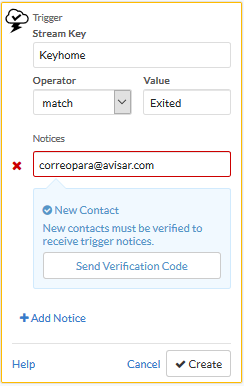
\includegraphics[scale = 0.8]{fig/Configuracion-de-aviso.PNG}
\caption{Configuración de aviso en la plataforma InitialState}
\label{fig:aviso-personalizado}
\end{figure}

En la figura~\ref{fig:sensor-detector-distancia} puede observarse como se crea un aviso, en el caso de que en la monitorización llamada Keyhome, se produzca una interrupción del funcionamiento (Exited), se informará del suceso al correo que se indica. De esta manera, el anfitrión tendrá la seguridad, en todo momento, de que su sistema se encuentra en funcionamiento, y de que, en caso de que algún programa falle, tendrá conocimiento de ello y podrá actuar en consecuencia.

Una vez que todas las debilidades tenidas en cuenta han sido consideradas a nivel de software, llega el momento de realizar un diseño que convierta este proyecto en un prototipo también a nivel físico. Para ello, se ha llevado a cabo el desarrollo de una caja donde se almacenará el circuito electrónico que incluye la Raspberry Pi, el sensor de proximidad, el conversor de niveles lógicos y el relé.

Para llevar a cabo el diseño de este prototipo, se ha hecho uso de la aplicación Autodesk Fusion 360\footnote{\url{https://www.autodesk.com/products/fusion-360/overview}}, la cual permite realizar diseños en tres dimensiones que posteriormente pueden ser impresos.

La función de este dispositivo es, principalmente, garantizar los niveles mínimos de seguridad a nivel físico, evitando que la Raspberry Pi o cualquier otro elemento pueda ser manipulado. Además, esta proporciona un mayor atractivo visual al dispositivo, haciendo que resulte más llamativo a nivel comercial.

En las figuras ~\ref{fig:imagen-1-diseno-3d}, ~\ref{fig:imagen-2-diseno-3d}, ~\ref{fig:imagen-3-diseno-3d}, ~\ref{fig:imagen-4-diseno-3d} y ~\ref{fig:imagen-5-diseno-3d} puede observarse, en distintos ángulos, el aspecto físico que se ha proporcionado a este dispositivo.

\begin{figure}[tbp]
\centering
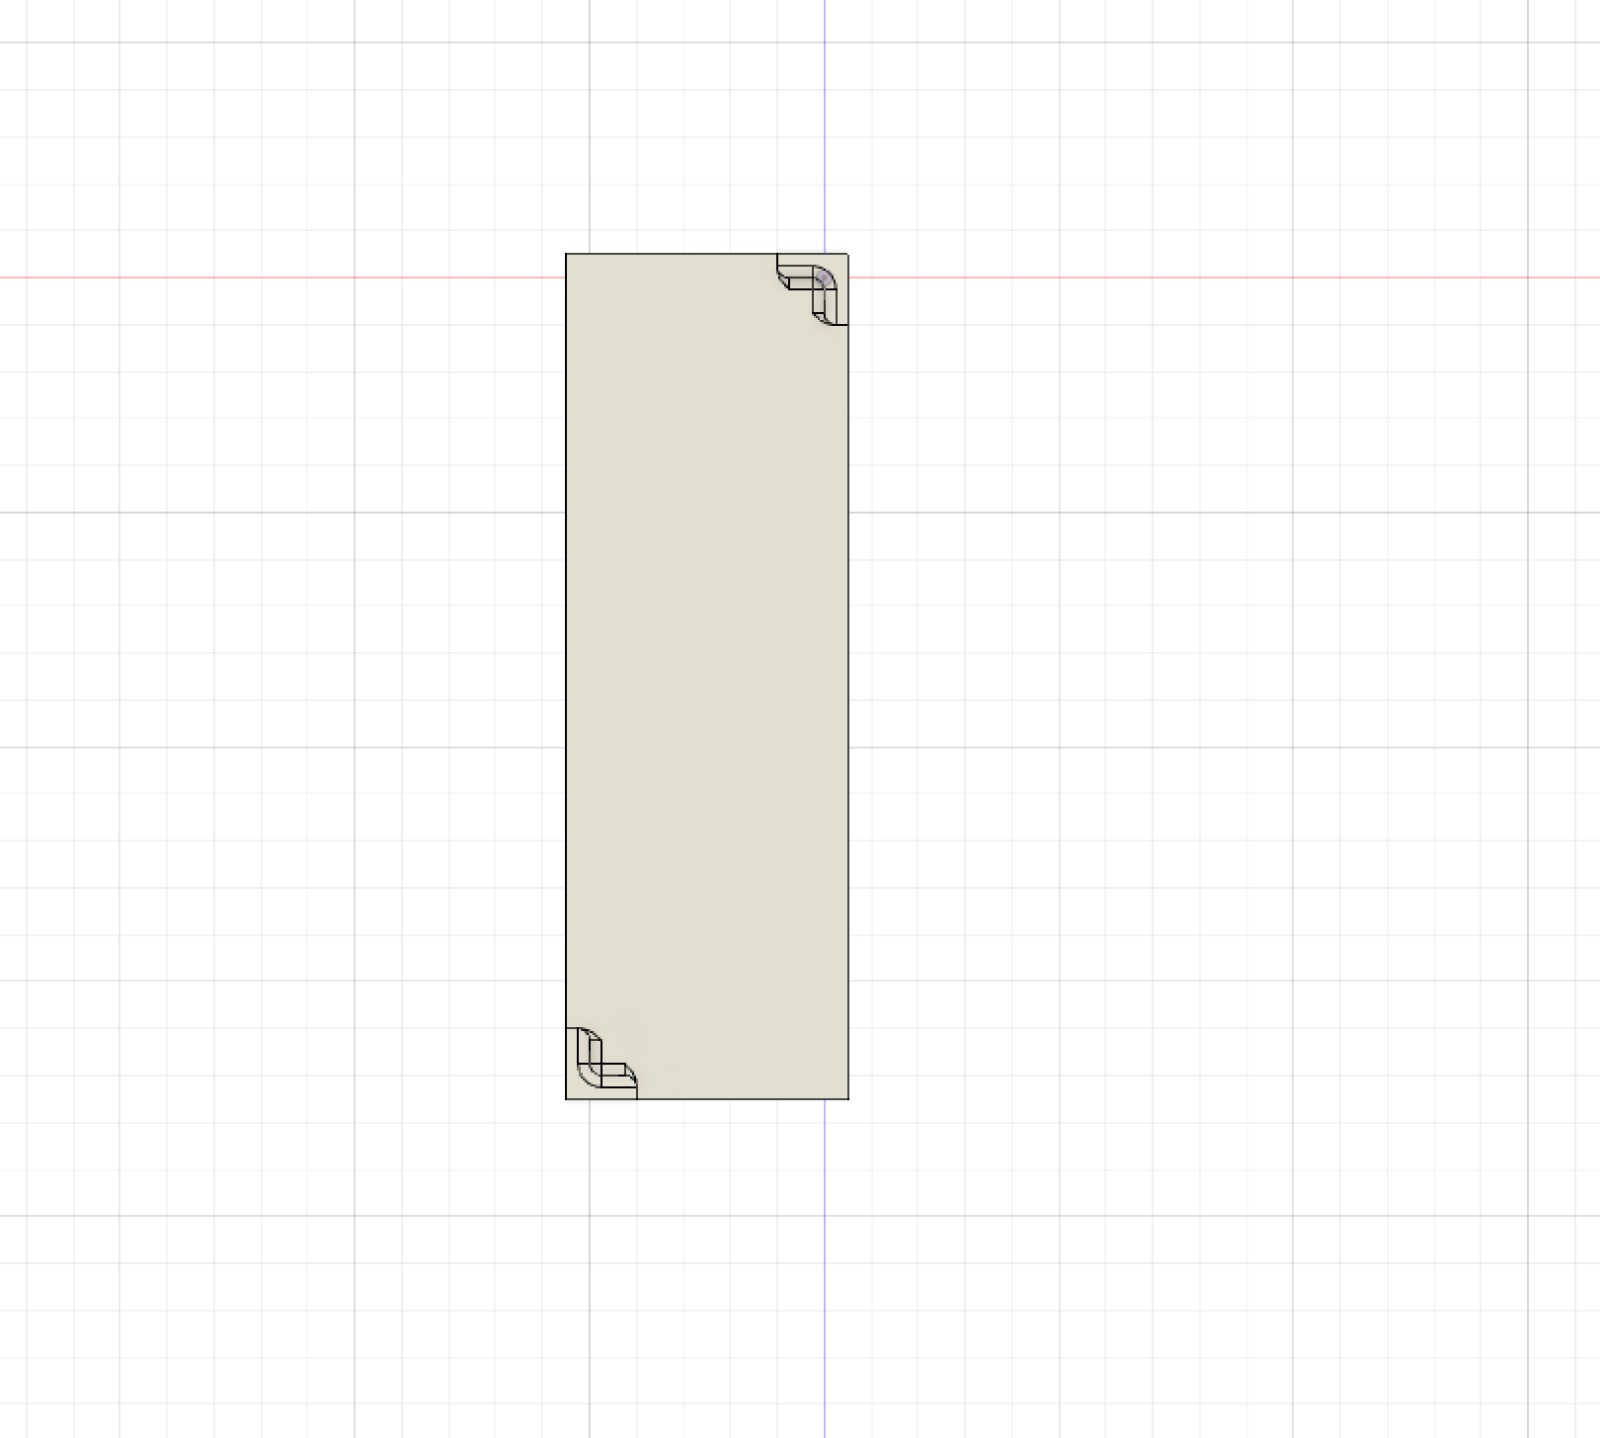
\includegraphics[scale = 0.2]{fig/Imagen_1_diseno_3D.jpeg}
\caption{Imagen 1 del diseño en 3D}
\label{fig:imagen-1-diseno-3d}
\end{figure}

\begin{figure}[tbp]
\centering
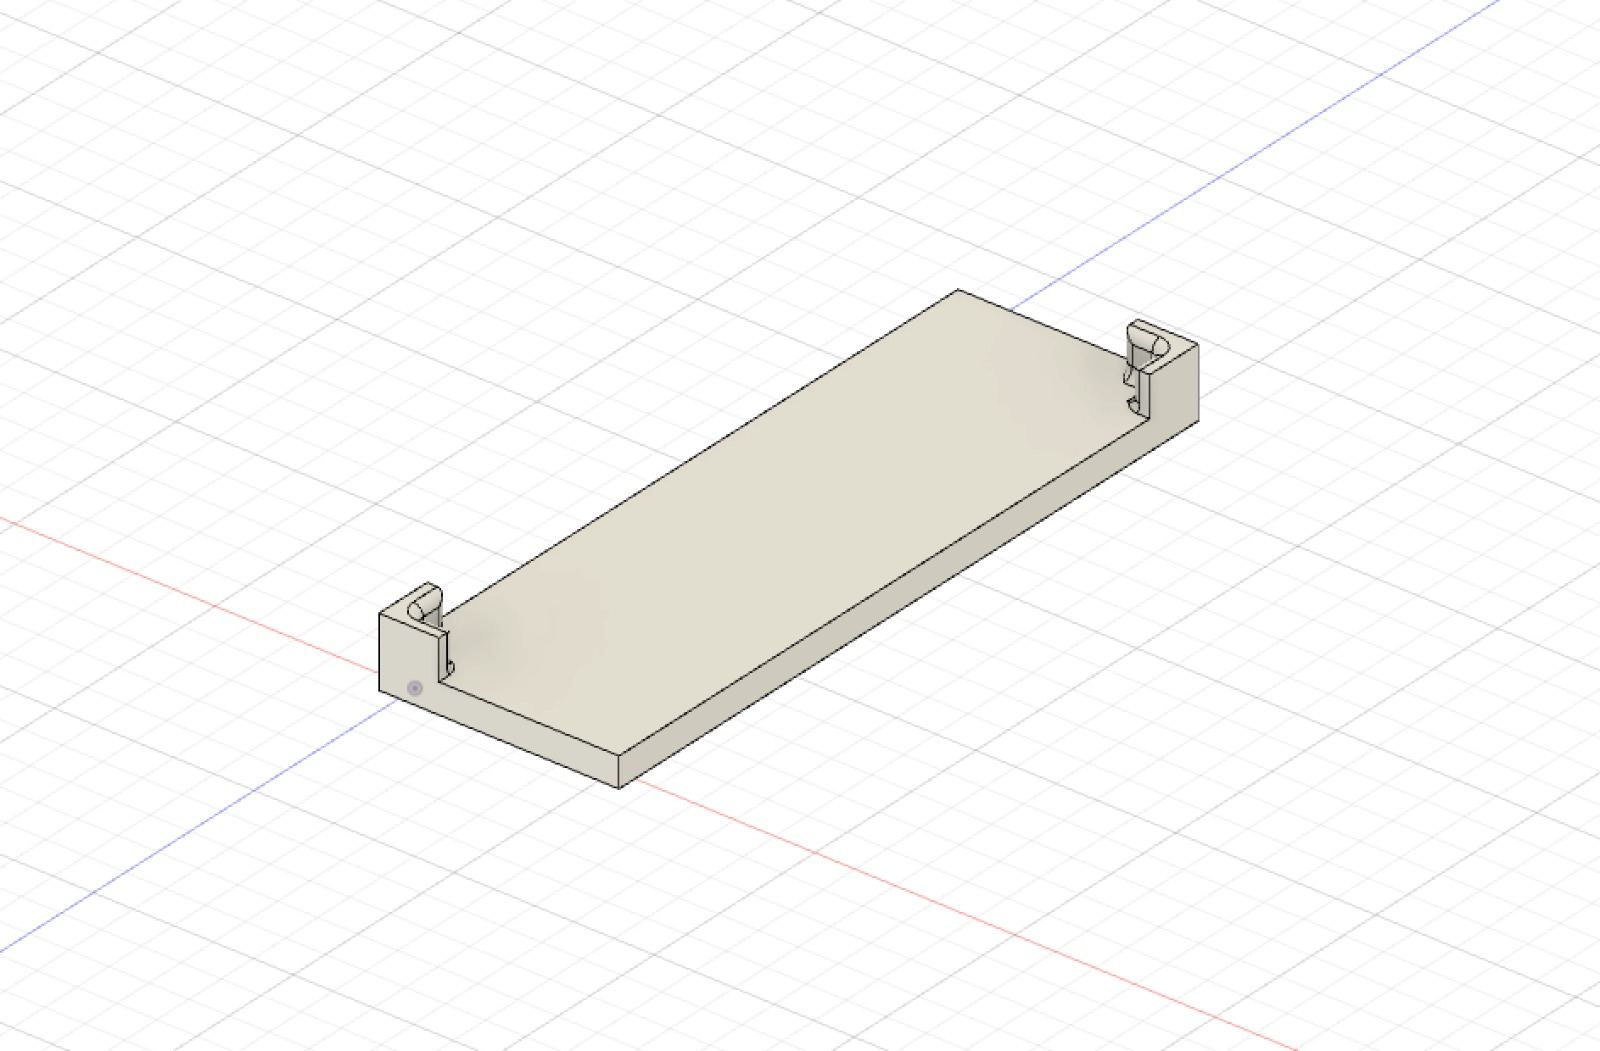
\includegraphics[scale = 0.2]{fig/Imagen_2_diseno_3D.jpeg}
\caption{Imagen 2 del diseño en 3D}
\label{fig:imagen-2-diseno-3d}
\end{figure}

\begin{figure}[tbp]
\centering
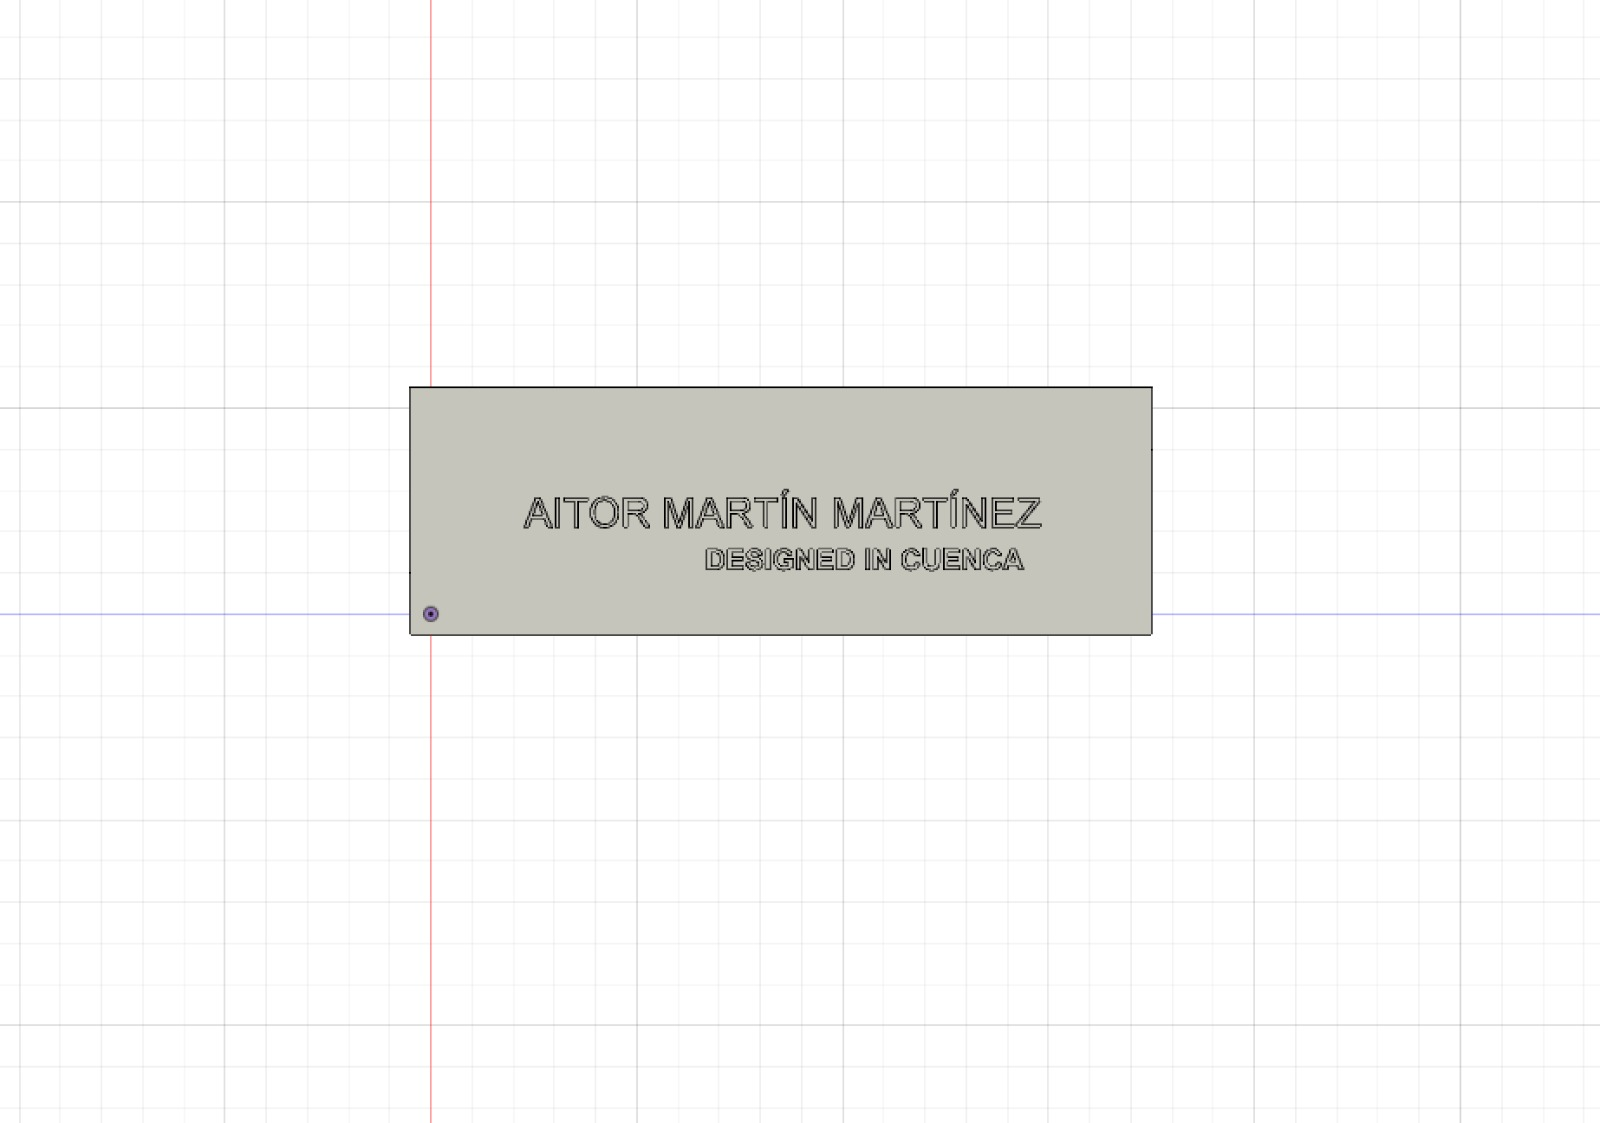
\includegraphics[scale = 0.2]{fig/Imagen_3_diseno_3D.jpeg}
\caption{Imagen 3 del diseño en 3D}
\label{fig:imagen-3-diseno-3d}
\end{figure}

\begin{figure}[tbp]
\centering
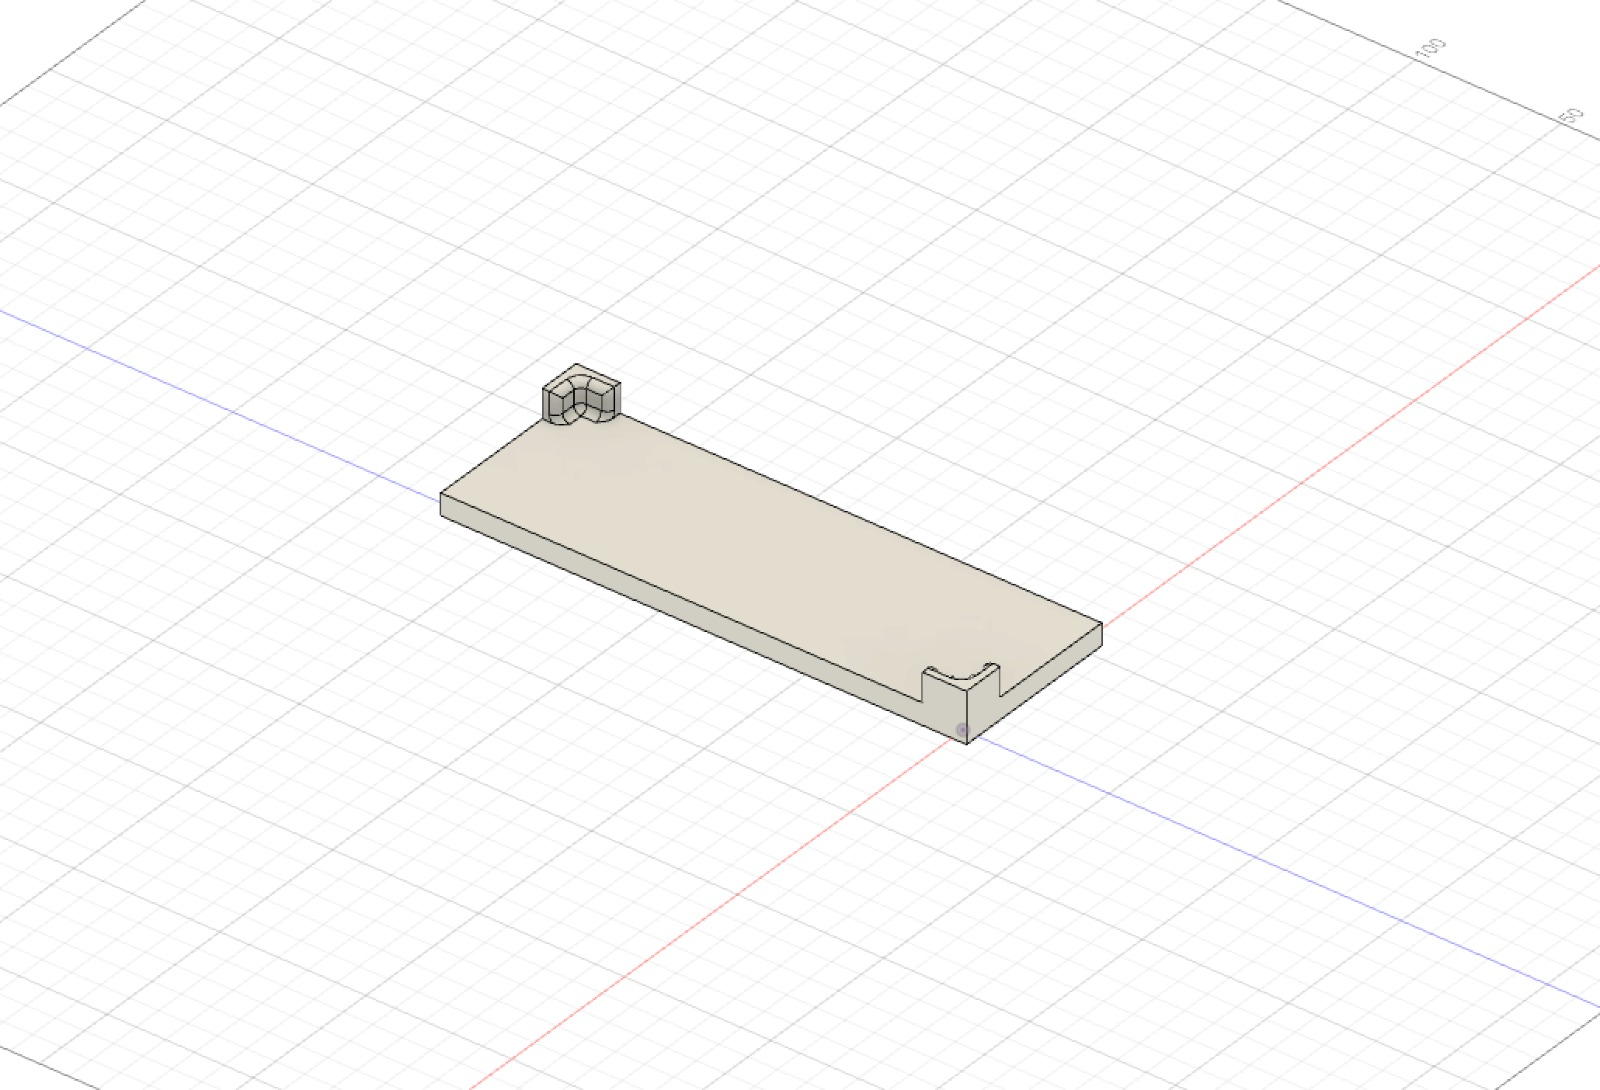
\includegraphics[scale = 0.2]{fig/Imagen_4_diseno_3D.jpeg}
\caption{Imagen 4 del diseño en 3D}
\label{fig:imagen-4-diseno-3d}
\end{figure}

\begin{figure}[tbp]
\centering
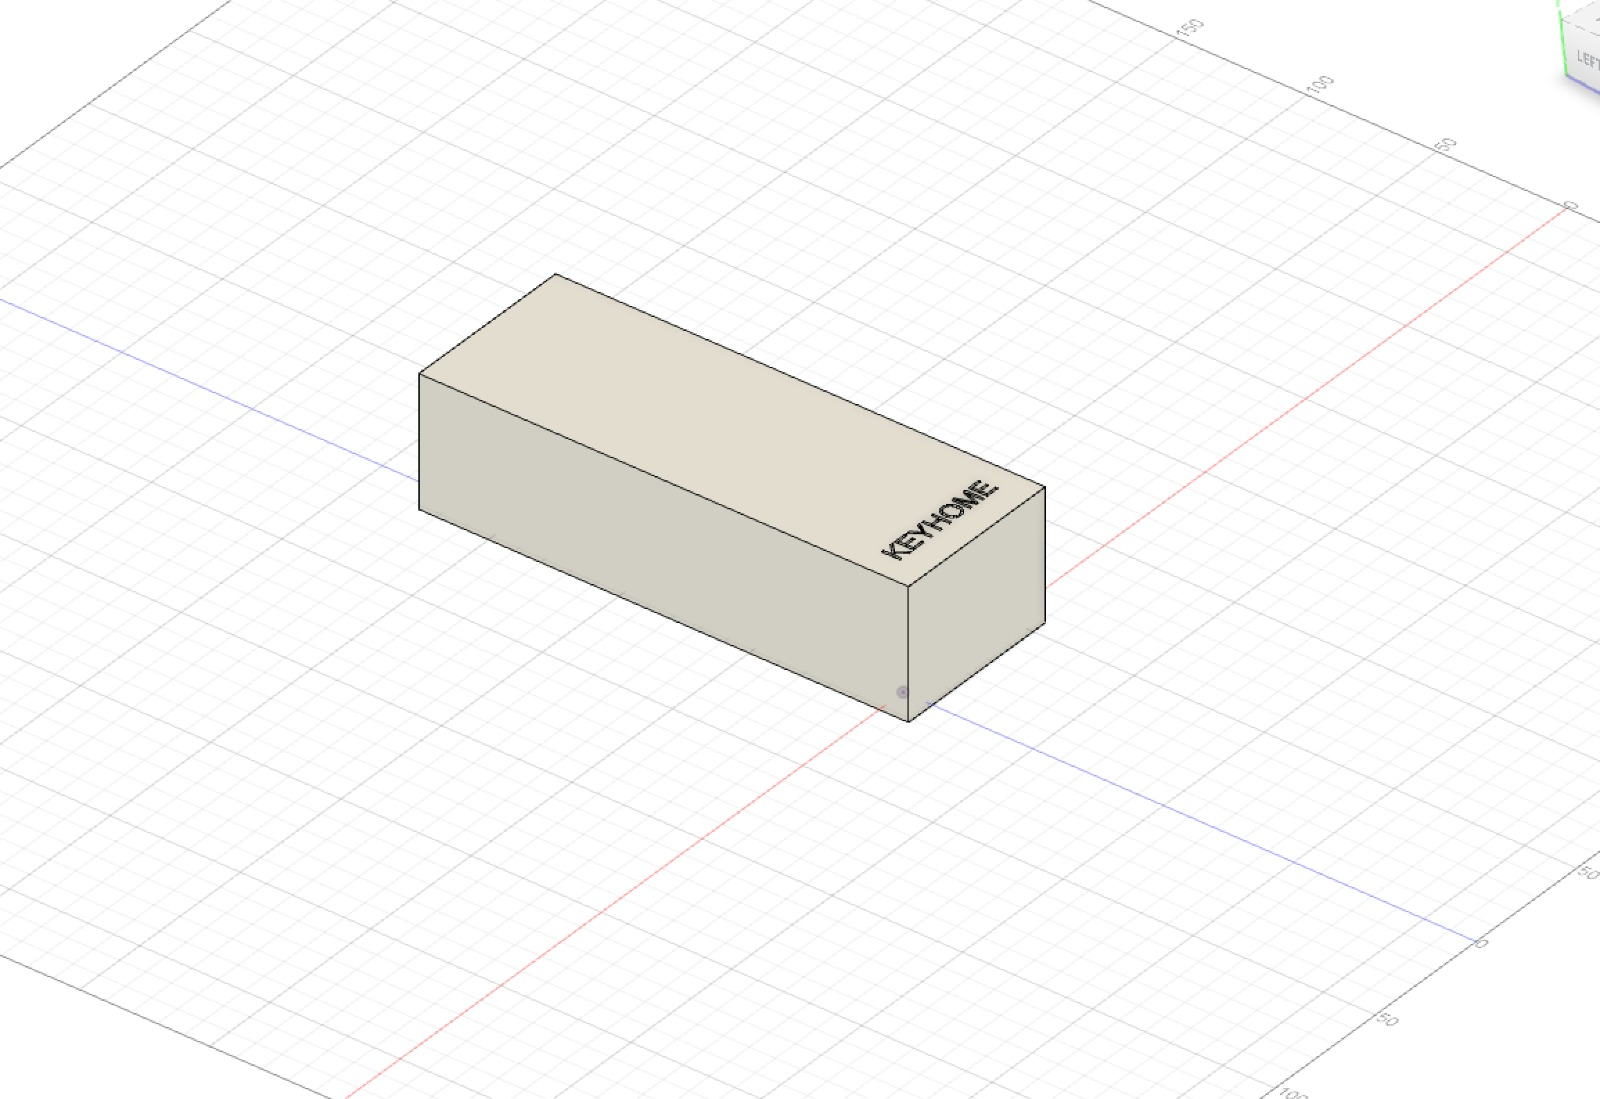
\includegraphics[scale = 0.2]{fig/Imagen_5_diseno_3D.jpeg}
\caption{Imagen 5 del diseño en 3D}
\label{fig:imagen-5-diseno-3d}
\end{figure}

Para que el proyecto funcione de forma correcta, este prototipo que contiene el circuito electrónico en su interior, deberá ser conducido hacia las conexiones realizadas en el portero automático que fueron explicadas en el primer apartado de este capitulo. Para conectar el interior del prototipo con el exterior, se hará uso de unos micro insertos roscados, que tienen un coste muy bajo y permiten incorporar estas conexiones de forma posterior a la impresión del prototipo.

Prestando atención a la figura~\ref{fig:imagen-2-diseno-3d}, puede observarse como la base de este dispositivo cuenta con dos esquinas ligeramente levantadas respecto al nivel del resto de la base. Con el fin de evitar, en la medida de lo posible, que intrusos abran el dispositivo, estos puntos serán perforados, junto con la tapa, por medio de un taladro que permitirá anclar un candado y cerrar de forma segura el dispositivo final. En la figura~\ref{fig:imagen-5-diseno-3d} se observa el aspecto visual que tendrá este dispositivo, una vez instalado en la vivienda.